\chapter{Structural Patterns in Pin-Wise MGXS}
\label{chap:spatial}

first paragraph: segue from preceding chapter
-previous chapter showed the benefit of using degenerate homogenization to best predict reaction rates sensitive to spatial self-shielding, most notably U-238 capture
-also highlighted issues of degenerate homognenization
  -large number of materials / large \ac{MGXS} datasets for deterministic multi-group codes
  -slow \ac{MC} convergence rate of \ac{MGXS} - low track density
-previous chapter noted that the error spatial distributions had structure - e.g., pins with similar neighbors generally had similar errors
  -this is an opportunity!!!

second paragraph: chapter objectives
-state chapter objectives:
  -analyze \ac{MGXS} data to identify structure -- namely, clustering -- of \ac{MGXS}
  -apply deterministic clustering technique for spatial homogenization
    -based on OpenCG \ac{LNS} algorithm - akin to a ``geometric template''
  -analyze the impact of \ac{LNS} homogenization with respect to the null and degenerate approaches from the last Chapter
  -motivate the need for a more flexible unsupervised approach

third paragraph: outline
-Sec.~\ref{sec:chap9-clustering} presents visualizations of clustering patterns in \ac{MGXS}
  -includes histograms in Sec.~\ref{subsec:chap9-histograms} and quantile-quantile plots in Sec.~\ref{subsec:chap9-qq-plots}
  -Sec.~\ref{subsec:chap9-clustering} shows the population variance for pin-wise \ac{MGXS}
-Sec.~\ref{sec:chap9-lns-homogenize} introduces \ac{LNS} spatial homogenization scheme
-Sec.~\ref{sec:chap9-lns-results} presents eigenvalues, fission rates and U-238 capture rates with \ac{LNS} spatial homogenization
-Sec.~\ref{sec:chap9-convergence} highlights the convergence rate of \ac{MGXS} computed using null, degenerate and \ac{LNS} spatial homogenization
-this chapter informs/motivates the need for an unsupervised approach to pin-wise spatial homogenization as discussed in the following chapter

%%%%%%%%%%%%%%%%%%%%%%%%%%%%%%%%%%%%%%%%%%%%%%%%%%%%%%%%%%%%%%%%%%%%%%%%%%%%%%%
\section{Clustering of Pin-Wise MGXS}
\label{sec:chap9-clustering}

first paragraph: postulate existence of clusters
-use infinite lattice example as ``thought experiment''
  -the \ac{MGXS} estimates for each pin from \ac{MC} tallies for an inf. lattice will be samples from a normal distribution
-spatial self-shielding experienced by different fuel pins induces clustering in pin-wise MGXS
  -i.e., differential moderation from \acp{CRGT} perturbs/softens flux in nearby pins
  -this affects the \ac{MGXS} in certain energy groups for certain nuclides
-explain why clustering only occurs for micro xs rather than macro
  -only way to compare differential impact of self-shielding on different pins is with micros
  -the macros will necessarily ``cluster'' according to nuclide density
  
second paragraph: intro to visualizations
-can be informative to illustrate \ac{MGXS} clusters with an exploration of the data through visualizations
-introduce infinite lattice geometries w/o \acp{CRGT} and w/o \acp{BP}
-section looks at different types of visualizations to understand
-note that although we identified U-238 capture \ac{MGXS} as being more impacted by pin-wise spatial homogenization in the last chapter, we present visualizations of U-235 fission here
  -other reaction rates may also be used to identify clustering in \ac{MGXS}
  -even if the clusters in those \ac{MGXS} don't make as much of an impact for their respective reaction types (e.g., fission vs. capture)

third paragraph: outline
-Sec.~\ref{subsec:chap9-pop-var} - population variance of \ac{MGXS} in each benchmark
-Sec.~\ref{subsec:chap9-histograms} - histograms plots of pin-wise \ac{MGXS}
  -for both U-238 capture and U-235 fission
  -although 
-Sec.~\ref{subsec:chap9-qq-plots} - quantile-quantile plots of pin-wise \ac{MGXS}

%%%%%%%%%%%%%%%%%%%%%%%%%%%%%%%%%%%%%%%%%%%%%%
\subsection{Pin-Wise MGXS Population Variance}
\label{subsec:chap9-pop-var}

first paragraph: heterogeneities induce a dispersion of pin-wise \ac{MGXS}
-hypothesize that 
  -evidence from degenerate scheme in preceding chapter backs this up
-Tab.~\ref{table:chap9-pop-var-mgxs} shows the population variance of pin-wise \ac{MGXS}
  -each sample in the population represents a single fuel pin
    -used OpenMC distributed cell tallies
  -for each benchmark, for both 1.6\% and 3.1\% enriched fuel pins
  	-note that there are 2.4\% enriched fuel pins in the \ac{BEAVRS} quarter core model
  -for group 1/2 U-238 capture \ac{MGXS}
  -for group 2/2 U-235 fission \ac{MGXS}

second paragraph: identify trends
-following sections seek to characterize structure in the dispersion of \ac{MGXS}
-inf lattice vs. not
  -dispersion / variance is over two orders of magnitude larger with the presence of heterogeneities
    -for same \ac{MC} track density and uncertainties for each pin's \ac{MGXS}
    -for both fission and capture 
-by fission vs. capture rxns
-by GTs
  -presence of GTS increases dispersion by two orders of magnitude
-by BPs
  -adding BPs actually slightly reduces dispersion of both capture \ac{MGXS}
  -increases dispersion by nearly 3$\times$ for fission \ac{MGXS}
-by enrichment
  -dispersion is greater for 3.1\% enr. pins - esp. for fission - over 2$\times$ larger!! 
    -e.g., 6.78 vs. 16.8 barns for 1.6\% and 3.1\% enr. pins in the \ac{BEAVRS} quarter core)
    -fission \ac{MGXS} is more sensitive to self-shielding
    -BUT fission rxn rates were not improved with degenerate homogenization
      -perhaps fission is still useful to identify clusters to improve U-238 capture predictions
-inter-assembly
  -increases capture dispersion by 10--20\%
  -increases fission dispersion by 5$\times$ (wrt assms w/o BPs) 
-by reflector
  -increases capture dispersion 5--15\%
  -increases fission dispersion by 60\% and over 100\% for 1.6\% and 3.1\% enr. fuel 
-by BEAVRS
  -dispersion decreases for BEAVRS wrt colorset w/ reflector by 1/2 -- 1/3 
  -dispersion increases slightly for U-238 capture in 3.1\% enr. fuel

%-plot the convergence of null MGXS by batch along with max for distribcell MGXS
%-plot the pop. var. convergence of the distribcell MGXS and show that they don't go to zero

\begin{table}[h!]
  \centering
  \caption[Population variance for pin-wise MGXS]{The population variance for pin-wise fission and U-238 capture \ac{MGXS}.}
  \small
  \label{table:chap9-pop-var-mgxs}
  \vspace{6pt}
  \begin{tabular}{C{2.5cm} l C{2.5cm} C{2.5cm}}
  \toprule
  \rowcolor{lightgray}
  \multicolumn{1}{C{2.5cm}}{\textbf{Fuel Enrichment}} & \multicolumn{1}{c}{\textbf{Benchmark}} & \boldmath$\mathrm{Var}\left[\sigma_{c}^{U-238}\right]$ \textbf{[barns]} & \boldmath$\mathrm{Var}\left[\sigma_{f}\right]$ \textbf{[barns]} \\
  \toprule
\multirow{5}{*}{1.6\%} & Assm. (no \acp{CRGT}, no \acp{BP}) & 6.29E-07 & 5.06E--03 \\
& Assm. (no \acp{BP}) & 1.61E-04 & 1.81E+00 \\
& 2$\times$2 Colorset & 1.89E-04 & 1.18E+01 \\
& 2$\times$2 Colorset w/ Reflector & 2.03E-04 & 1.93E+01 \\
& \ac{BEAVRS} Quarter Core & 1.64E-04 & 6.78E+00 \\
\midrule
\multirow{6}{*}{3.1\%} & Assm. (no \acp{CRGT}, no \acp{BP}) & 5.83E-07 & 6.12E--03 \\
& Assm. (no \acp{BP}) & 1.53E-04 & 4.22E+00 \\
& Assm. (20 \acp{BP}) & 1.37E-04 & 1.11E+01 \\
& 2$\times$2 Colorset & 1.53E-04 & 2.15E+01 \\
& 2$\times$2 Colorset w/ Reflector & 1.79E-04 & 4.78E+01 \\
& \ac{BEAVRS} Quarter Core & 2.34E-04 & 1.68E+01 \\
\bottomrule
\end{tabular}
\end{table}

%%%%%%%%%%%%%%%%%%%%%%%%%%%%%%%%%%%%%%%%
\subsection{Histograms of Pin-Wise MGXS}
\label{subsec:chap9-histograms}

first paragraph: histograms and rug plots
-describe what a histrogram is?
-describe what a rug plot is
-construct plots for each benchmark
-construct plots of the U-238 capture (group 1/2) and U-235 fission (group 2/2) \ac{MGXS} in each pin
  -the ``samples'' in the plots each correspond to a single fuel pin instance
    -i.e., each green mark in the rug plots represents a single fuel pin
-could clearly have looked at other reactions, groups, nuclides
  -for brevity, selected just a few which largely govern reactor performance to present here
  -could have selected data from more groups, but it is ``noisier''
    -the trends are not as easy to identify as they are for 2-group data

%%%%%%%%%%%%%%%%%%%%%%%%%%%%%%%
\subsubsection{U-238 Capture MGXS}
\label{subsubsec:chap9-histograms-capt}

first paragraph: intro U-238 capture \ac{MGXS} histograms
-Fig.~\ref{fig:chap9-hist-1.6-capt} and ~\ref{fig:chap9-hist-3.1-capt}
  -U-238 capture \ac{MGXS} for 1.6\% and 3.1\% enriched fuel pins
  -in each of the heterogeneous benchmarks, respectively
-recall these are micro xs
-recall the inf. lattice case

second paragraph: trends w/ enrichment:
-generally 1.6\% enr. is 0.01-0.02 barns larger
  -micros for inf. lattice are $\sim$ 0.01 barns larger for 1.6\% than 3.1\% enr.
  -micros for lattice w/ \acp{CRGT} are $\sim$ 0.01 barns larger for 1.6\% than 3.1\% enr.
  -micros for 2$\times$2 colorsets are $\sim$0.01-0.02 barns larger for 1.6\% than 3.1\% enr.
  -micros for full core vary over wider range for 3.1\% enr.
    -extend to over 0.9 barns for a few pins
    -while 0.87 is the highest of any 1.6\% enr. pin in the full core
    -the micros for the 3.1\% enriched pins are typically a few hundredths of a barn larger 

third paragraph: analyze trends
-trends w/ \acp{CRGT}
  -addition of \acp{CRGT} induces four clearly discernible clusters
  -separated by $\sim$0.1-0.15 barns for both 1.6\% and 3.1\% enriched pins
  -potentially may be sub-clusters, especially b/w smallest two clusters
    -in range of 0.8-0.81 barns and 0.79-0.8 barns for 1.6\%/3.1\% enriched pins, respectively
  -four cases in order of increasing degree of flux softening due to differential moderation:
    -not adjacent to \ac{CRGT}
    -corner adjacent to \ac{CRGT}
    -facially adjacent to \ac{CRGT}
    -facially and corner adjacent to two separate \acp{CRGT}

-trends w/ \acp{BP}
  -addition of \acp{BP} for 3.1\% enr. assm ``smears'' clusters
  -seems to shift \ac{MGXS} down by $\sim$0.005 barns wrt case w/o \acp{BP}
  -still seem to be four distinct clusters, but more liklely 6+ clusters
  
-trends w/ inter-assembly interface (2$\times$2 colorset w/o reflector)
  -``smearing'' of clusters
  -important to recognize that there are now 264 times 2 = 528 samples
    -expect it to be more difficult to discern clusters from rug plot with more samples
  -still seem to be four distinct clusters for 1.6\% enriched fuel pins
    -largest cluster is $\sim$0.01 barn higher at 0.85 barns
  -more difficult to discern clusters for 3.1\% enr. pins, but appears to be at least 3
    -all \ac{MGXS} shifted down by $\sim$0.0075 barns 

-trends w/ reflector
  -recall which assm is where in the configuration
    -3.1\% w/ 20 \acp{BP} are adjacent to reflector
    -1.6\% w/o \acp{BP} are on the interior and corner adjacent to reflector
  -still 3 strong clusters for 1.6\% enr. pins
    -more ``smeared'', especially on the low side where
    -a few pins have \ac{MGXS} as low as $\sim$0.76 barns
  -similar trends for the 3.1\% enr. pins
    -pins with smallest \ac{MGXS} shifted down by $\sim$0.025 barns
  
-trends with full core
  -recall how many pins of each type are in the full core
    -4236 3.1\% enriched
    -4332 1.6\% enriched
    -4260 2.4\% enriched
  -1.6\% enr. seems to have two peaks at 0.815 and 0.83 barns
  -3.1\% enr. seems to have two peaks at 0.785 and 0.805 barns
    -with a much smaller shoulder centered 0.83 barns
    -a few pins with much higher \ac{MGXS} b/w 0.86 and 0.9 barns
  -\ac{MGXS} are not generally dispersed any more than they were for the colorsets
  

SUMMARY BOX

-think about shifts in \ac{MGXS} in terms of percentages

\begin{figure}[h!]
\centering
\begin{subfigure}{0.5\textwidth}
  \centering
  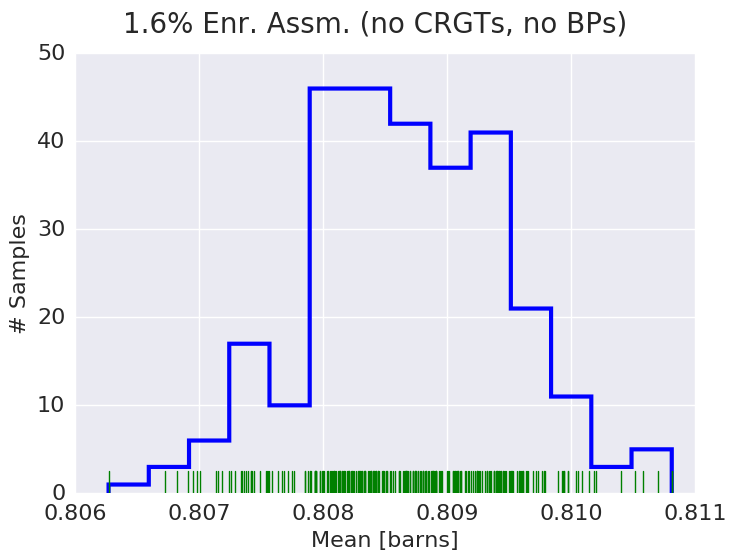
\includegraphics[width=\linewidth]{figures/patterns/assm-1.6-inf/hist-kde-rug/assm-16-inf-capt-1}
  \caption{}
  \label{fig:chap9-hist-assm-1.6-inf-capt}
\end{subfigure}%
\begin{subfigure}{0.5\textwidth}
  \centering
  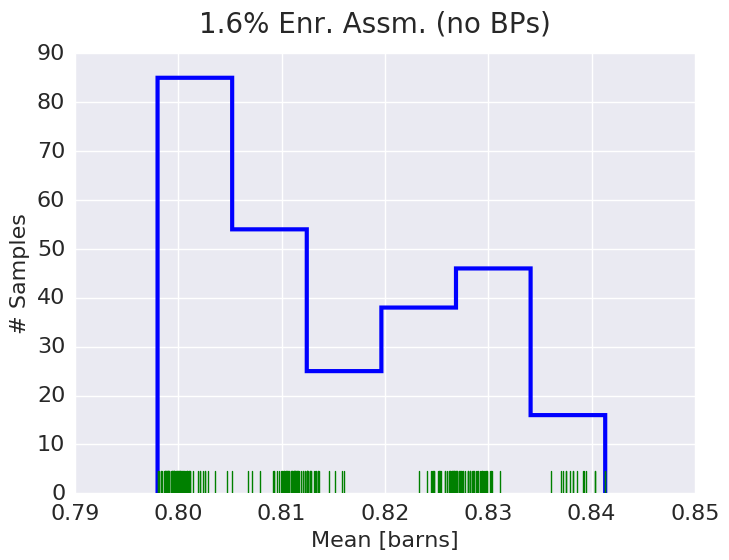
\includegraphics[width=\linewidth]{figures/patterns/assm-1.6/hist-kde-rug/assm-16-capt-1}
  \caption{}
  \label{fig:chap9-hist-assm-1.6-capt}
\end{subfigure}
\begin{subfigure}{0.5\textwidth}
  \centering
  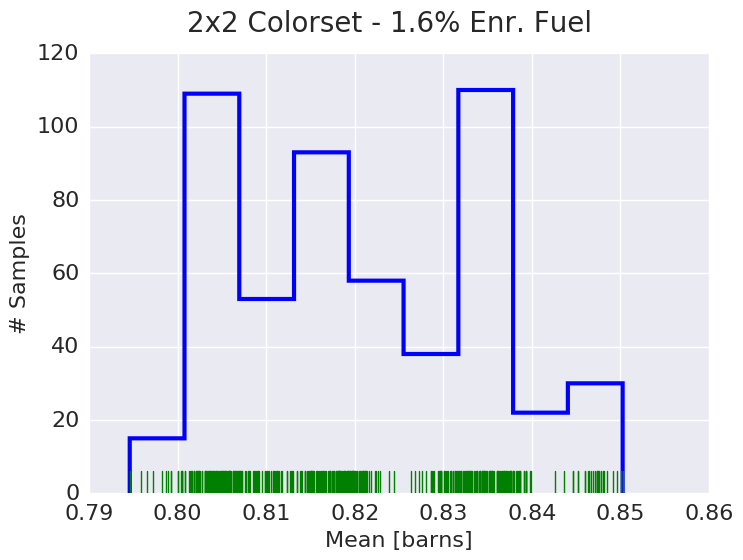
\includegraphics[width=\linewidth]{figures/patterns/2x2/hist-kde-rug/16-enr-capt-1}
  \caption{}
  \label{fig:chap9-hist-2x2-1.6-capt}
\end{subfigure}%
\begin{subfigure}{0.5\textwidth}
  \centering
  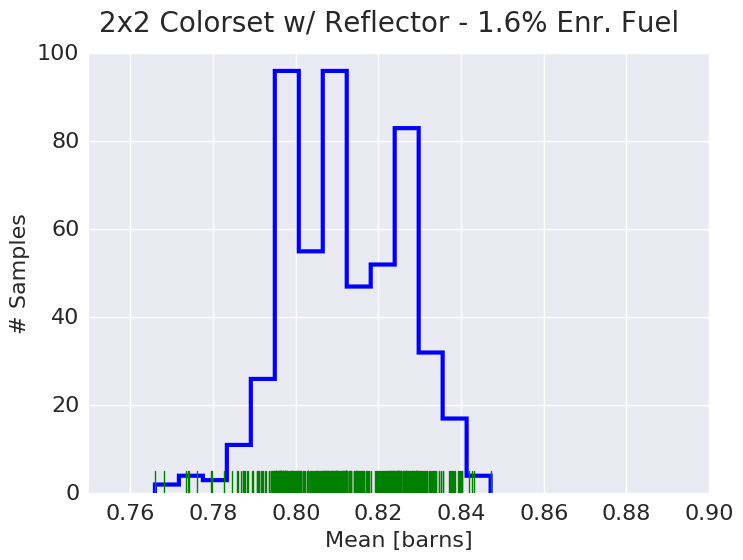
\includegraphics[width=\linewidth]{figures/patterns/reflector/hist-kde-rug/16-enr-capt-1}  \caption{}
  \label{fig:chap9-hist-reflector-1.6-capt}
\end{subfigure}
\begin{subfigure}{0.5\textwidth}
  \centering
  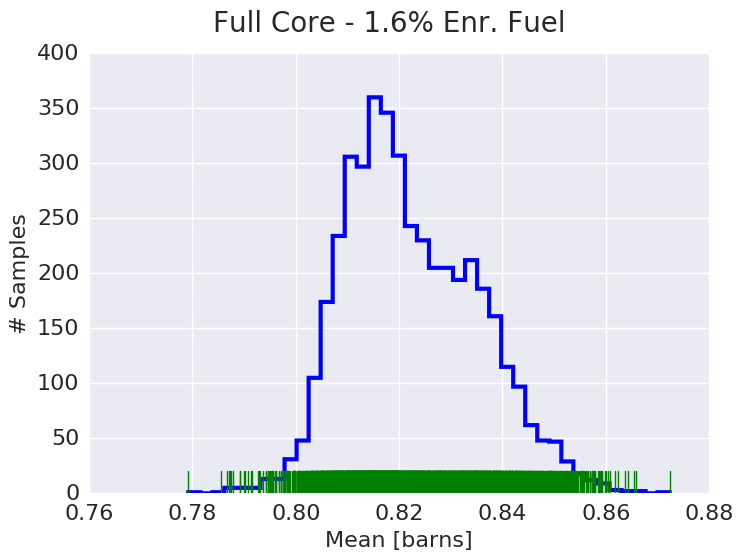
\includegraphics[width=\linewidth]{figures/patterns/full-core/hist-kde-rug/16-enr-capt-1} \caption{}
  \label{fig:chap9-hist-full-core-1.6-capt}
\end{subfigure}
\caption[Histogram of U-238 capture MGXS for 1.6\% enriched fuel]{Histograms of U-238 capture \ac{MGXS} (group 1 of 2) for 1.6\% enriched fuel.}
\label{fig:chap9-hist-1.6-capt}
\end{figure}

\begin{figure}[h!]
\centering
\begin{subfigure}{0.5\textwidth}
  \centering
  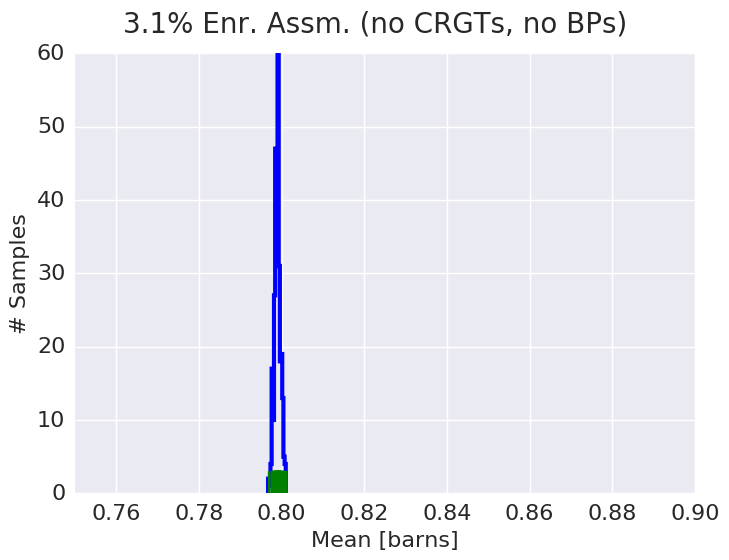
\includegraphics[width=\linewidth]{figures/patterns/assm-3.1-inf/hist-kde-rug/assm-31-inf-capt-1}
  \caption{}
  \label{fig:chap9-hist-assm-3.1-inf-capt}
\end{subfigure}%
\begin{subfigure}{0.5\textwidth}
  \centering
  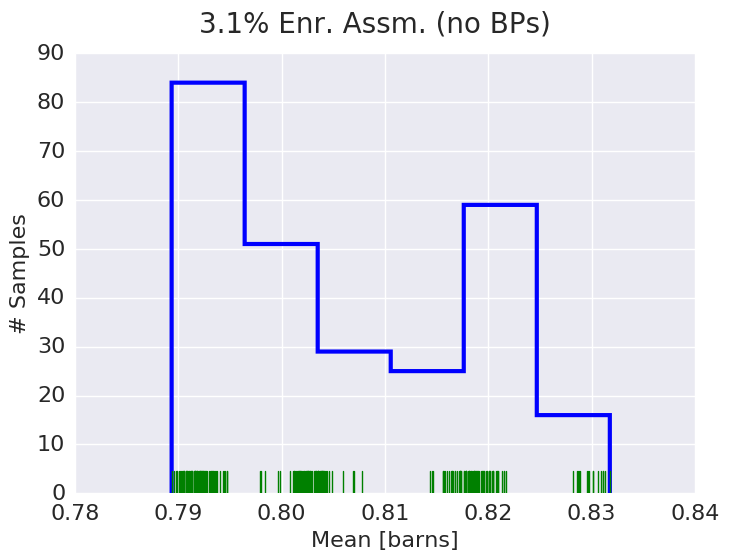
\includegraphics[width=\linewidth]{figures/patterns/assm-3.1/hist-kde-rug/assm-31-capt-1}
  \caption{}
  \label{fig:chap9-hist-assm-3.1-capt}
\end{subfigure}
\begin{subfigure}{0.5\textwidth}
  \centering
  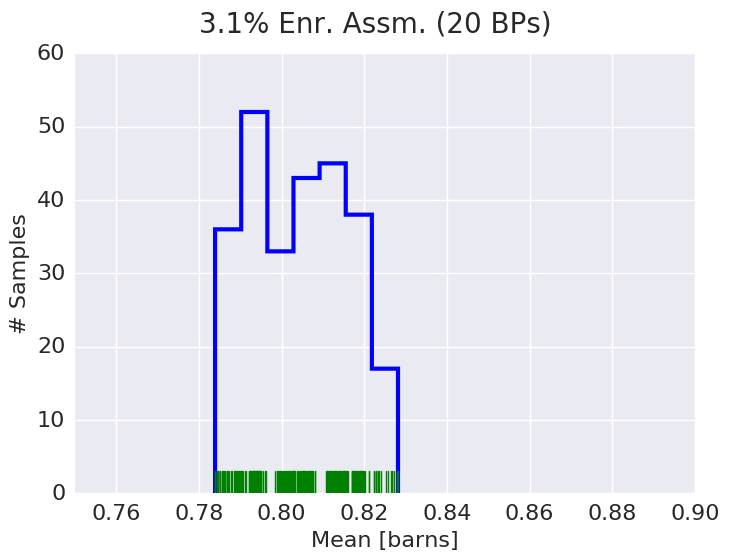
\includegraphics[width=\linewidth]{figures/patterns/assm-3.1-20BPs/hist-kde-rug/assm-31-20BPs-capt-1}
  \caption{}
  \label{fig:chap9-hist-assm-3.1-20BPs-capt}
\end{subfigure}%
\begin{subfigure}{0.5\textwidth}
  \centering
  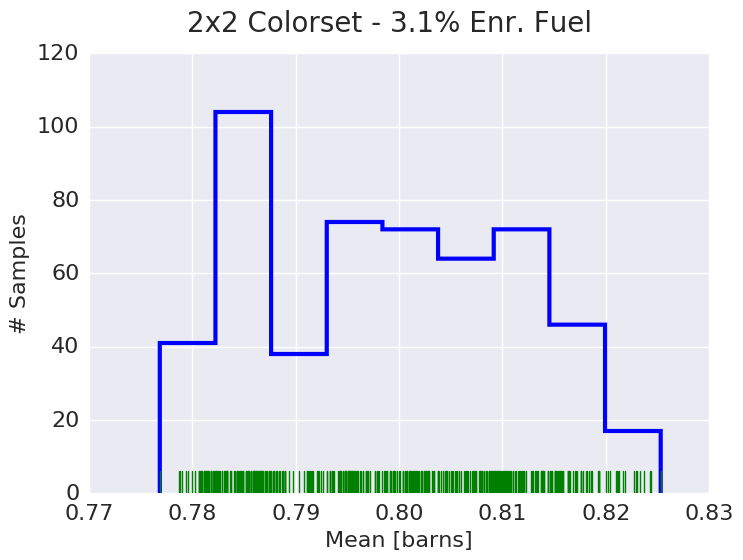
\includegraphics[width=\linewidth]{figures/patterns/2x2/hist-kde-rug/31-enr-capt-1}
  \caption{}
  \label{fig:chap9-hist-2x2-3.1-capt}
\end{subfigure}
\begin{subfigure}{0.5\textwidth}
  \centering
  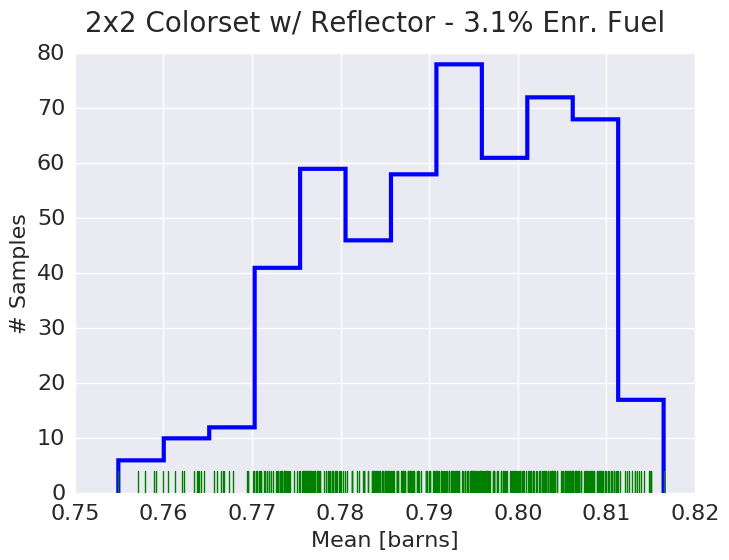
\includegraphics[width=\linewidth]{figures/patterns/reflector/hist-kde-rug/31-enr-capt-1}  \caption{}
  \label{fig:chap9-hist-reflector-3.1-capt}
\end{subfigure}%
\begin{subfigure}{0.5\textwidth}
  \centering
  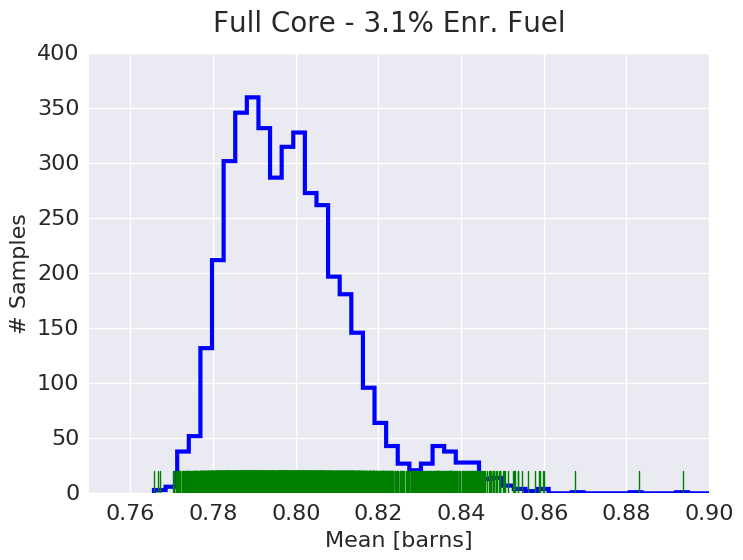
\includegraphics[width=\linewidth]{figures/patterns/full-core/hist-kde-rug/31-enr-capt-1} \caption{}
  \label{fig:chap9-hist-full-core-3.1-capt}
\end{subfigure}
\caption[Histogram of U-238 capture MGXS for 3.1\% enriched fuel]{Histograms of U-238 capture \ac{MGXS} (group 2 of 2) for 3.1\% enriched fuel.}
\label{fig:chap9-hist-3.1-capt}
\end{figure}

%%%%%%%%%%%%%%%%%%%%%%%%%%%%%%%%%%
\subsubsection{U-235 Fission MGXS}
\label{subsubsec:chap9-histograms-fiss}

first paragraph: intro U-235 fission \ac{MGXS} histograms
-Fig.~\ref{fig:chap9-hist-1.6-fiss} and ~\ref{fig:chap9-hist-3.1-fiss}
  -U-235 fission \ac{MGXS} for 1.6\% and 3.1\% enriched fuel pins
  -in each of the heterogeneous benchmarks, respectively
-recall these are micro xs
-recall the inf. lattice case
-micro U-235 \ac{MGXS} for fission is over 300$\times$ larger than U-238 capture \ac{MGXS}
  -BUT the nuclide density for U-238 is over 30--60$\times$ larger than U-235 for 1.6\% and 3.1\% enriched fuel, respectively
  -hence, clustering for micro U-238 capture \ac{MGXS} is important even though the micro is much smaller
  -an error of 1\% in the \ac{MGXS} for either is problematic

second paragraph: trends w/ enrichment:
-generally 1.6\% enr. is 0.01-0.02 barns larger
  -micros for inf. lattice are $\sim$ 18 barns larger for 1.6\% than 3.1\% enr.
  -micros for lattice w/ \acp{CRGT} are $\sim$ 18 barns larger for 1.6\% than 3.1\% enr.
  -micros for 2$\times$2 colorsets are up to 22 barns larger for 1.6\% than 3.1\% enr.
  -micros for full core vary over wider range for 3.1\% enr.
    -extend up to 305 barns for a few 1.6\% enr. pins, but only 287.5 barns for 3.1\% enr. pins
    -do not extend over as wide of a range as the 2$\times$2 colorset w/ reflector for either enr.

third paragraph: analyze trends
-trends w/ \acp{CRGT}
  -histograms indicate roughly 3 clusters for each enrichment
  -upper bound \ac{MGXS} are shifted up by more than 5 barns with \acp{CRGT} (nearly 2\%)
  -rug plots tell a more complicated story
    -the data is more ``smeared'' across the range than for U-238 capture
    -clusters appear to be more distinct for 3.1\% enrichment - coincidence???
      -seem to be about 8 clusters, tougher to tell for 1.6\% enrichment
      -regardless, seems to be more sensitive to other self-shielding / differential moderation effects than U-238 capture
        -BUT the total range of MGXS varies by only 1.3\% as compared to 5\% for U-238 capture

-trends w/ \acp{BP}
  -shifts lower bound down by 9 barns (3\%)
  -shifts upper bound down by 4 barns (1.3\%)
  -appear to be 3 strong clusters centered at 272, 276 and 300 barns (w/ sub-clusters)
    -adjacent clusters differ by $\sim$1.3\%
  -addition of \acp{BP} makes clusters more distinct (unlike for U-238)
  
-trends w/ inter-assembly interface (2$\times$2 colorset w/o reflector)
  -seems to be 3 and 4 strong clusters for 1.6\% and 3.1\% enriched pins (based on histograms)
    -centered at 294, 298 and 301 barns for 1.6\% enr
    -centered at 271, 275, 278 and 283 barns for 3.1\% enr
    -adjacent clusters differ by 1--2\%
  -rug plots indicate more clusters than this
  -clusters more distinguishable than they were for single assembly  
  -clusters are more distinguishable than they were for U-238 capture \ac{MGXS}
  -lower bound for 1.6\% enr. fuel is shifted down by $\sim$6 barns (2\%)
  -upper bound for 3.1\% enr. fuel is shifted up by $\sim$3 barns (1\%)

-trends w/ reflector
  -recall which assm is where in the configuration
    -3.1\% w/ 20 \acp{BP} are adjacent to reflector
    -1.6\% w/o \acp{BP} are on the interior and corner adjacent to reflector
  -structure is very different for the two enrichments
    -dispersion of a few pins with largest \ac{MGXS} of 15 barns greater than case w/o reflector (5\%)
  -roughly six clusters for 1.6\% enr. centered at 294, 298, 301, 304, 306, and 310 barns
    -largest cluster at 301 barns
    -certainly more sub-clusters
    -one pin with 315 barn \ac{MGXS} (cornermost pin with most added moderation from reflector)
  -rougly four clusters for 3.1\% enr. centered at 276, 284, 290 296 barns
    -largest cluster at 276 barrns
    -certainly more sub-clusters
  
-trends with full core
  -recall how many pins of each type are in the full core
    -4236 3.1\% enriched
    -4332 1.6\% enriched
    -4260 2.4\% enriched
  -1.6\% enr. seems to have two clearly defined peaks 297 and 302 barns
    -peaks are more clearly discernible than for 3.1\% enr.
  -3.1\% enr. seems to have three most clearly defined peaks at 278, 283 and 284 barns
  -both have \ac{MGXS} smeared across 15 barns (5\%) which is less than the 20--25 barns for the 2$\times$2 colorsets w/ a reflector and more similar to the range seen for the colorset w/o a reflector
  -range of \ac{MGXS} is are not generally dispersed any more than they were for the colorsets 

SUMMARY BOX

-think about shifts in \ac{MGXS} in terms of percentages

\begin{figure}[h!]
\centering
\begin{subfigure}{0.5\textwidth}
  \centering
  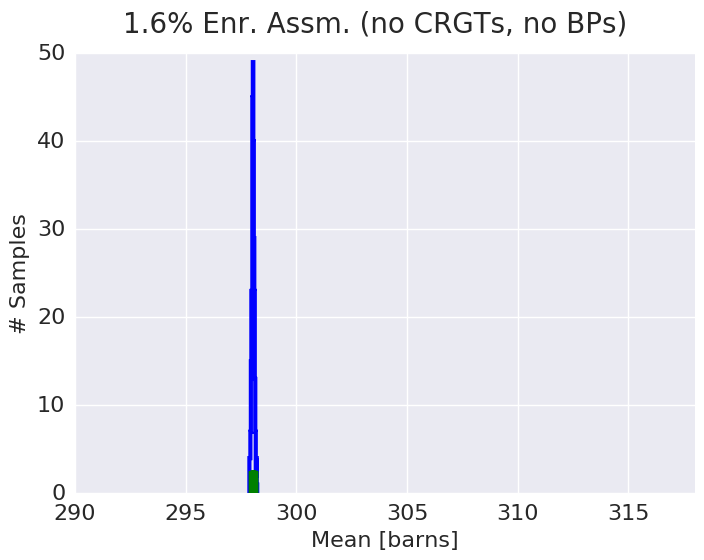
\includegraphics[width=\linewidth]{figures/patterns/assm-1.6-inf/hist-kde-rug/assm-16-inf-fiss-2}
  \caption{}
  \label{fig:chap9-hist-assm-1.6-inf-fiss}
\end{subfigure}%
\begin{subfigure}{0.5\textwidth}
  \centering
  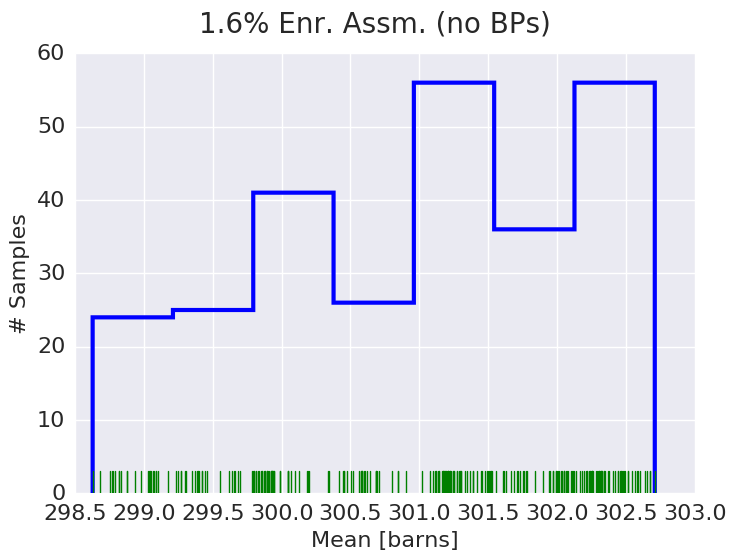
\includegraphics[width=\linewidth]{figures/patterns/assm-1.6/hist-kde-rug/assm-16-fiss-2}
  \caption{}
  \label{fig:chap9-hist-assm-1.6-fiss}
\end{subfigure}
\begin{subfigure}{0.5\textwidth}
  \centering
  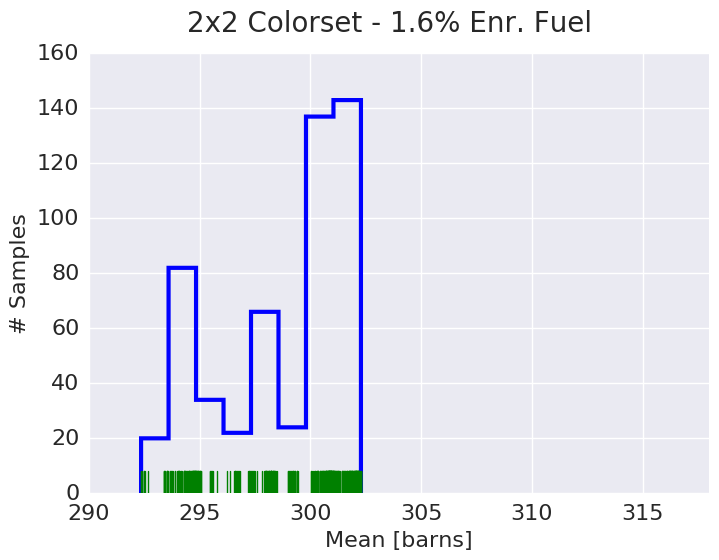
\includegraphics[width=\linewidth]{figures/patterns/2x2/hist-kde-rug/16-enr-fiss-2}
  \caption{}
  \label{fig:chap9-hist-2x2-1.6-fiss}
\end{subfigure}%
\begin{subfigure}{0.5\textwidth}
  \centering
  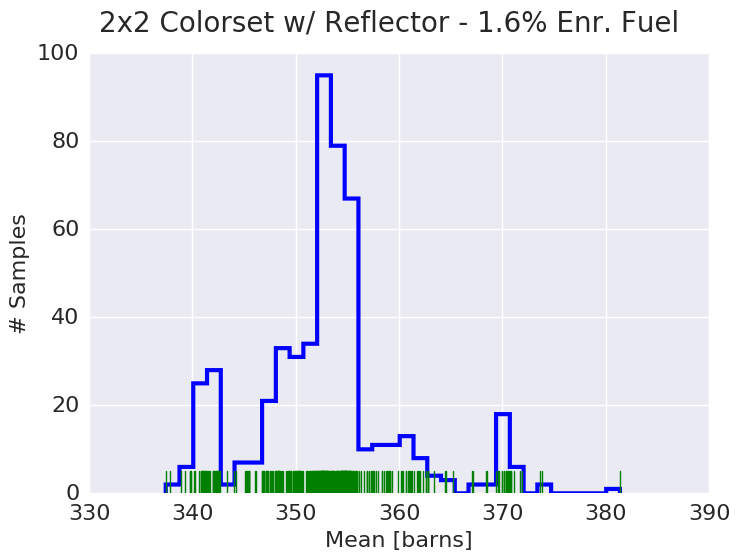
\includegraphics[width=\linewidth]{figures/patterns/reflector/hist-kde-rug/16-enr-fiss-2}  \caption{}
  \label{fig:chap9-hist-reflector-1.6-fiss}
\end{subfigure}
\begin{subfigure}{0.5\textwidth}
  \centering
  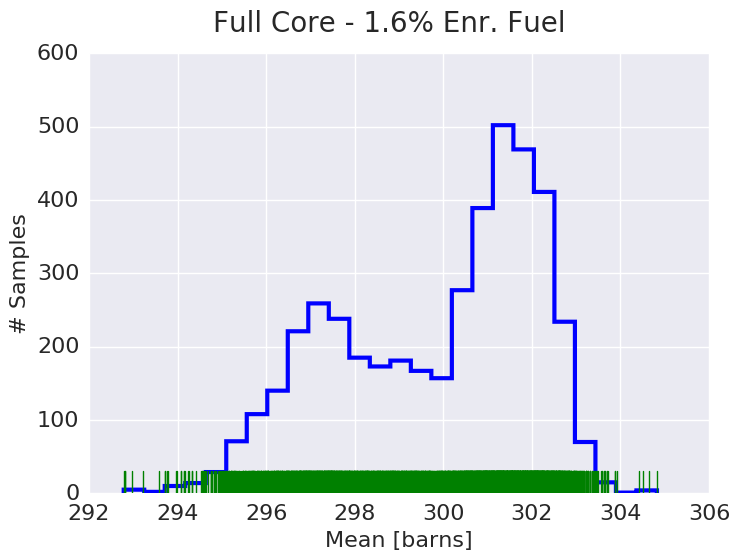
\includegraphics[width=\linewidth]{figures/patterns/full-core/hist-kde-rug/16-enr-fiss-2} \caption{}
  \label{fig:chap9-hist-full-core-1.6-fiss}
\end{subfigure}
\caption[Histogram of U-235 fission MGXS for 1.6\% enriched fuel]{Histograms of U-235 fission \ac{MGXS} (group 1 of 2) for 1.6\% enriched fuel.}
\label{fig:chap9-hist-1.6-fiss}
\end{figure}

\begin{figure}[h!]
\centering
\begin{subfigure}{0.5\textwidth}
  \centering
  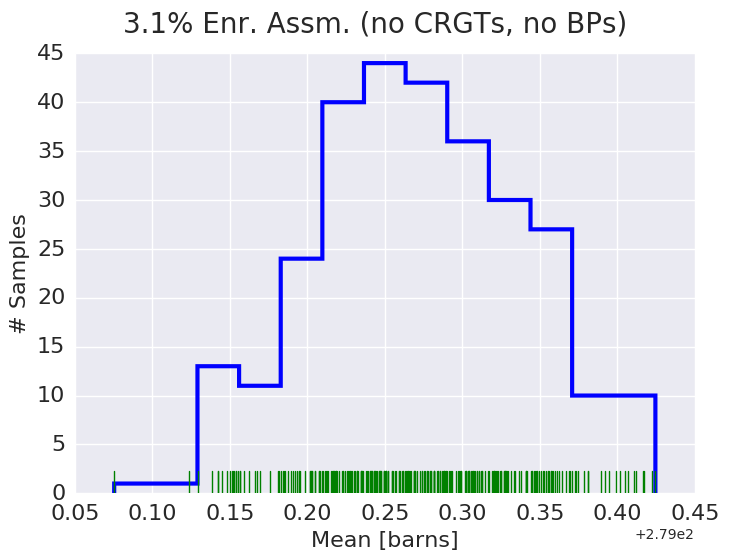
\includegraphics[width=\linewidth]{figures/patterns/assm-3.1-inf/hist-kde-rug/assm-31-inf-fiss-2}
  \caption{}
  \label{fig:chap9-hist-assm-3.1-inf-fiss}
\end{subfigure}%
\begin{subfigure}{0.5\textwidth}
  \centering
  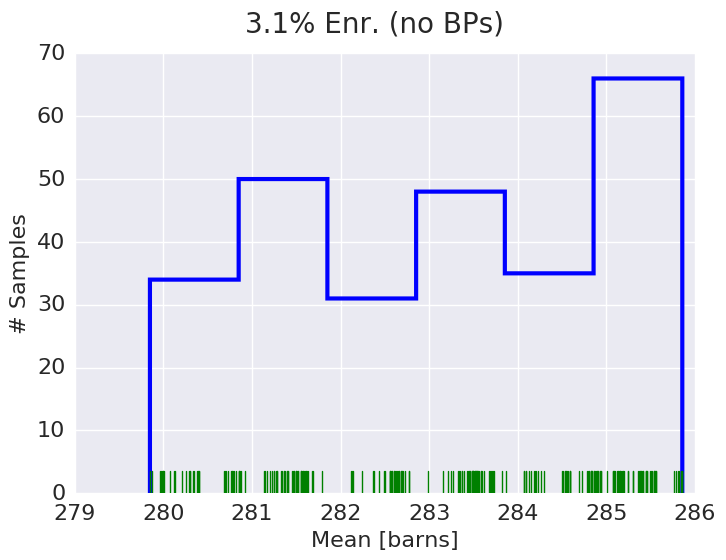
\includegraphics[width=\linewidth]{figures/patterns/assm-3.1/hist-kde-rug/assm-31-fiss-2}
  \caption{}
  \label{fig:chap9-hist-assm-3.1-fiss}
\end{subfigure}
\begin{subfigure}{0.5\textwidth}
  \centering
  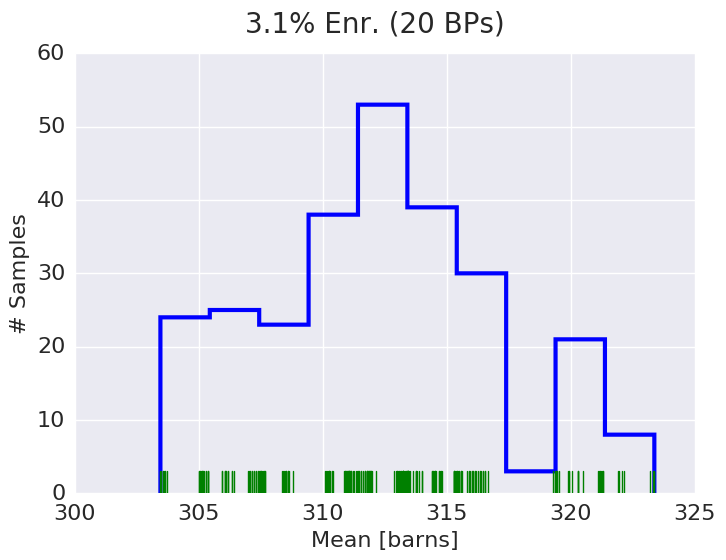
\includegraphics[width=\linewidth]{figures/patterns/assm-3.1-20BPs/hist-kde-rug/assm-31-20BPs-fiss-2}
  \caption{}
  \label{fig:chap9-hist-assm-3.1-20BPs-fiss}
\end{subfigure}%
\begin{subfigure}{0.5\textwidth}
  \centering
  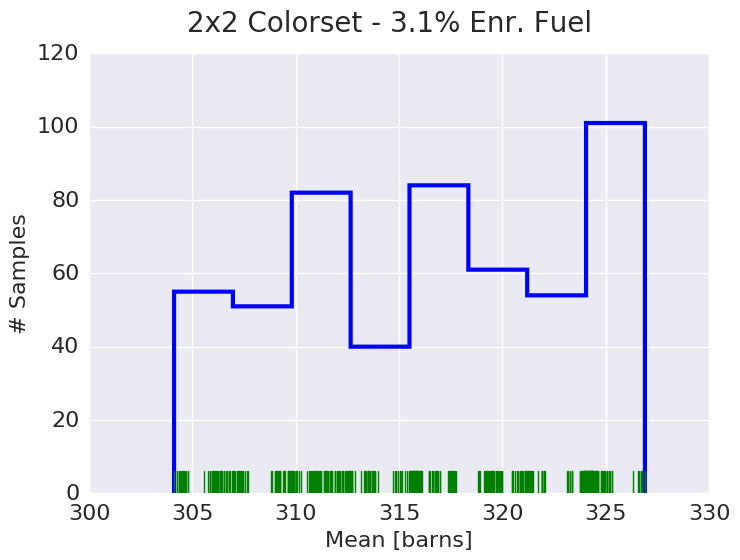
\includegraphics[width=\linewidth]{figures/patterns/2x2/hist-kde-rug/31-enr-fiss-2}
  \caption{}
  \label{fig:chap9-hist-2x2-3.1-fiss}
\end{subfigure}
\begin{subfigure}{0.5\textwidth}
  \centering
  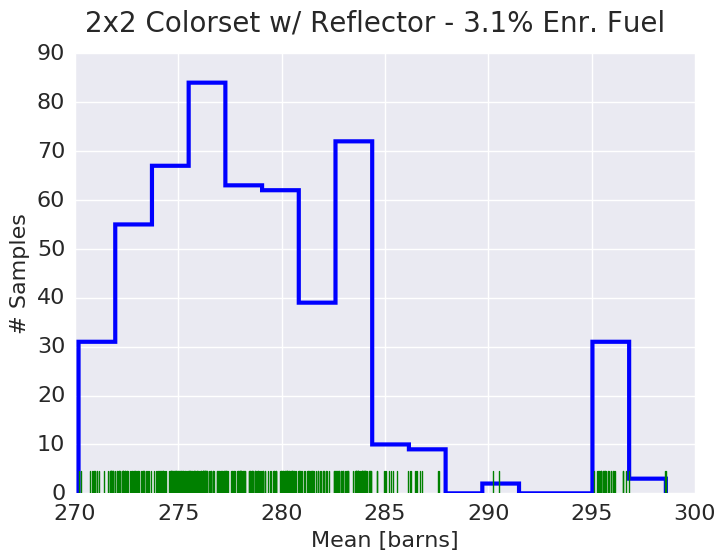
\includegraphics[width=\linewidth]{figures/patterns/reflector/hist-kde-rug/31-enr-fiss-2}  \caption{}
  \label{fig:chap9-hist-reflector-3.1-fiss}
\end{subfigure}%
\begin{subfigure}{0.5\textwidth}
  \centering
  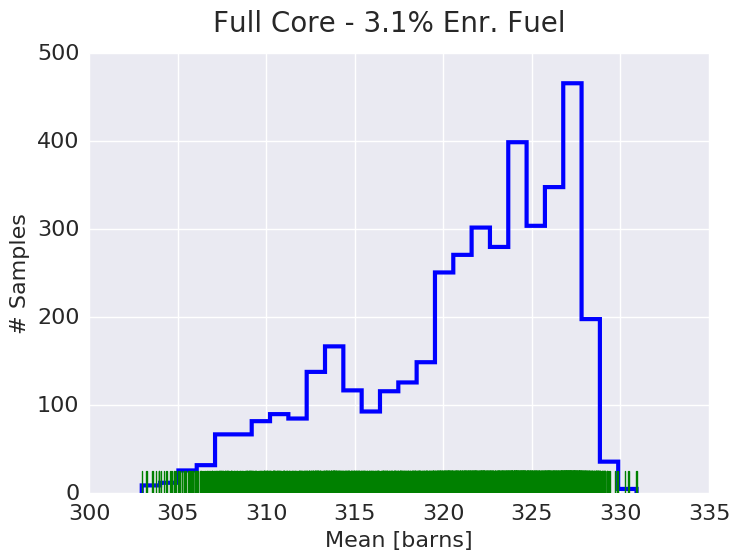
\includegraphics[width=\linewidth]{figures/patterns/full-core/hist-kde-rug/31-enr-fiss-2} \caption{}
  \label{fig:chap9-hist-full-core-3.1-fiss}
\end{subfigure}
\caption[Histogram of U-235 fission MGXS 3.1\% enriched fuel]{Histograms of U-235 fission \ac{MGXS} (group 2 of 2) for 3.1\% enriched fuel.}
\label{fig:chap9-hist-3.1-fiss}
\end{figure}


%%%%%%%%%%%%%%%%%%%%%%%%%%%%%%%%%%%%%%%%%%%%%%%%%%%%%
\subsection{Quantile-Quantile Plots of Pin-Wise MGXS}
\label{subsec:chap9-qq-plots}

first paragraph: qq plots
-describe what a qq plot is
-construct plots for each benchmark
-construct plots of the U-238 capture (group 1/2) and U-235 fission (group 2/2) \ac{MGXS} in each pin
  -the ``samples'' in the plots each correspond to a single fuel pin instance
    -i.e., each blue data point represents a single fuel pin
-could clearly have looked at other reactions, groups, nuclides
  -for brevity, selected just a few which largely govern reactor performance to present here
  -could have selected data from more groups, but it is ``noisier''
    -the trends are not as easy to identify as they are for 2-group data

second paragraph: normality tests
-explain what a p-value is
-reference shannon wilkes test or whatever in scipy


%%%%%%%%%%%%%%%%%%%%%%%%%%%%%%%%%%
\subsubsection{U-238 Capture MGXS}
\label{subsubsec:chap9-qq-plots-capt}

first paragraph: intro U-238 capture \ac{MGXS} qq plots
-Fig.~\ref{fig:chap9-qq-1.6-capt} and ~\ref{fig:chap9-qq-3.1-capt}
  -U-238 capture \ac{MGXS} for 1.6\% and 3.1\% enriched fuel pins
  -in each of the heterogeneous benchmarks, respectively
-recall the inf. lattice case

-second paragraph:
  -the qq plot shows that data for the inf. lattices very nearly normal (p-values well above 0.05, closer to 0.7)
  -clear deviation from normality with addition of \acp{CRGT}
  -structure is more challenging to understand for more complex benchmarks
    -addition of \acp{BP} for 3.1\% enr. assembly makes clusters/shoulders ``sharper'' steps
    -more data points (e.g., fuel pins) for each benchmark clouds the structure
	  -generally with more data points the trends are ``smoother''
	    -does NOT necessarily indicate better approx. to normality however!!
	    -``slow'' and ``smooth'' trends can still deviate widely from that expected for normal samples, e.g., 3.1\% enr. full core pin
  -p-value is very clearly smallest for the full core (1e-22 and 1e-39 for 1.6\% and 3.1\% enr fuel)

-mention that tails above and below on lower/upper range indicate that tails of distribution are not as wide as would be expected for normal samples -- e.g., a ``tighter'' or ``narrower'' distribution
-3.1\% enr pins in full core are tighter on bottom edge, but wider on upper edge
  -indicative of those few ``outlier'' pins with \ac{MGXS} near 0.9 barns in Fig.~\ref{fig:chap9-hist-3.1-capt}
  
SUMMARY BOX

-add ``Assm.'' to titles of plots for individual fuel assemblies
-add group 1/2 to captions

\begin{figure}[h!]
\centering
\begin{subfigure}{0.5\textwidth}
  \centering
  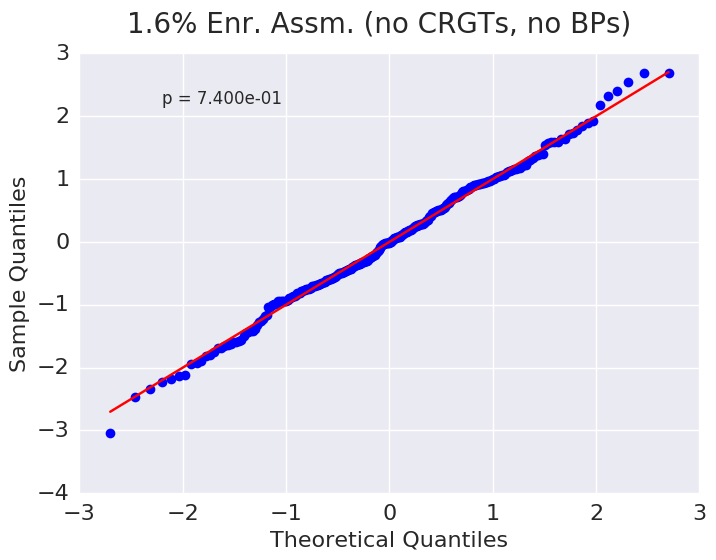
\includegraphics[width=\linewidth]{figures/patterns/assm-1.6-inf/quantile/assm-16-inf-capt-1}
  \caption{}
  \label{fig:chap9-qq-assm-1.6-inf-capt}
\end{subfigure}%
\begin{subfigure}{0.5\textwidth}
  \centering
  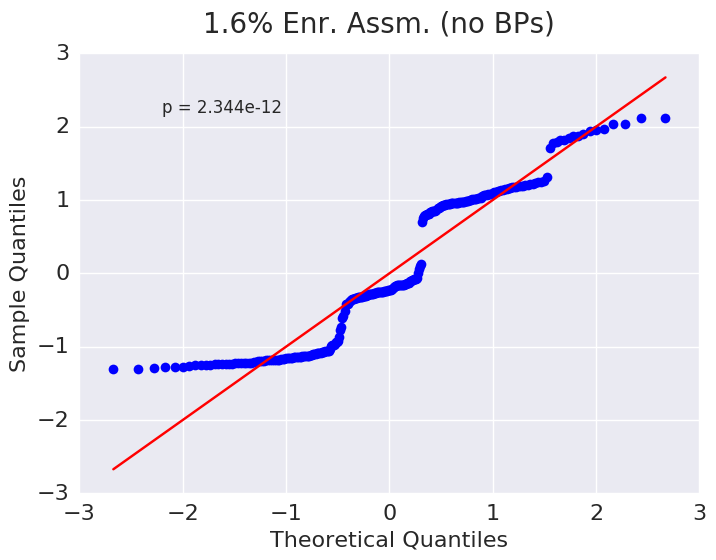
\includegraphics[width=\linewidth]{figures/patterns/assm-1.6/quantile/assm-16-capt-1}
  \caption{}
  \label{fig:chap9-qq-assm-1.6-capt}
\end{subfigure}
\begin{subfigure}{0.5\textwidth}
  \centering
  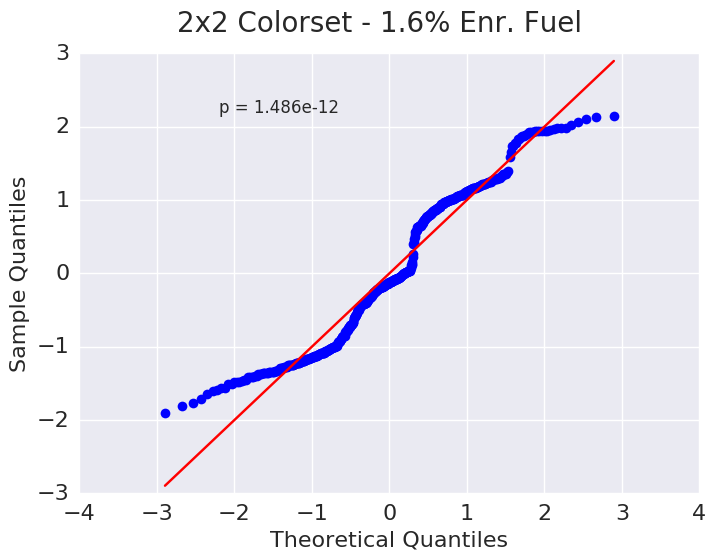
\includegraphics[width=\linewidth]{figures/patterns/2x2/quantile/16-enr-capt-1}
  \caption{}
  \label{fig:chap9-qq-2x2-1.6-capt}
\end{subfigure}%
\begin{subfigure}{0.5\textwidth}
  \centering
  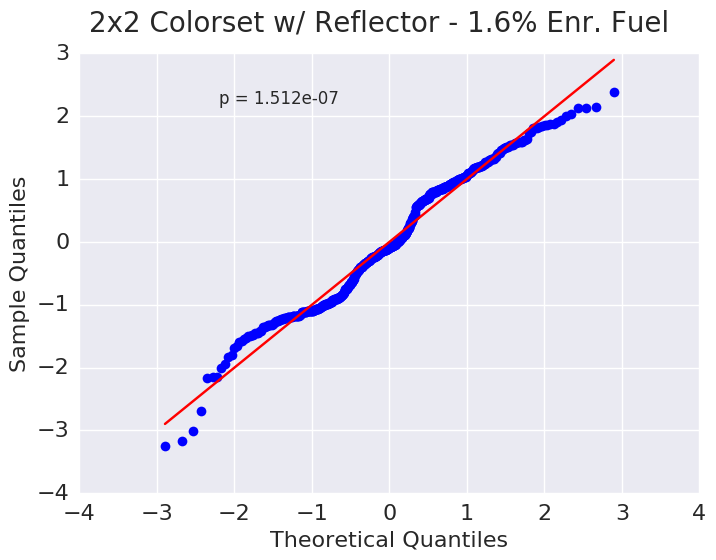
\includegraphics[width=\linewidth]{figures/patterns/reflector/quantile/16-enr-capt-1}  \caption{}
  \label{fig:chap9-qq-reflector-1.6-capt}
\end{subfigure}
\begin{subfigure}{0.5\textwidth}
  \centering
  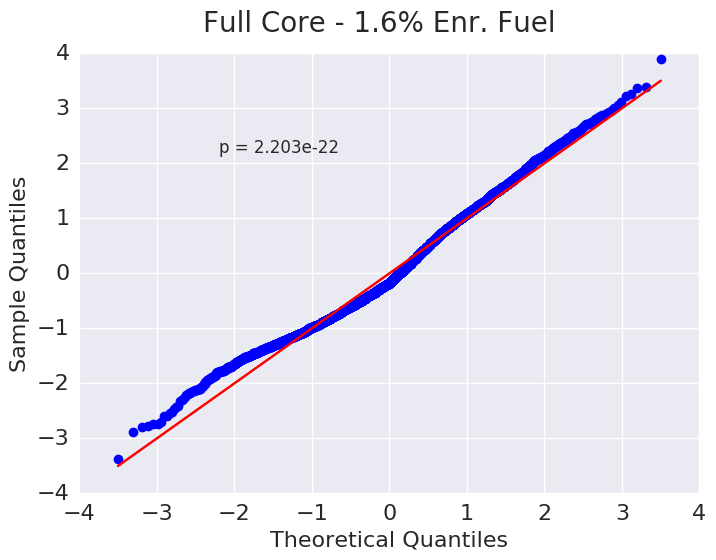
\includegraphics[width=\linewidth]{figures/patterns/full-core/quantile/16-enr-capt-1} \caption{}
  \label{fig:chap9-qq-full-core-1.6-capt}
\end{subfigure}
\caption[Q-Q plots of U-238 capture MGXS for 1.6\% enriched fuel]{Q-Q plots of U-238 capture \ac{MGXS} for 1.6\% enriched fuel.}
\label{fig:chap9-qq-1.6-capt}
\end{figure}

\begin{figure}[h!]
\centering
\begin{subfigure}{0.5\textwidth}
  \centering
  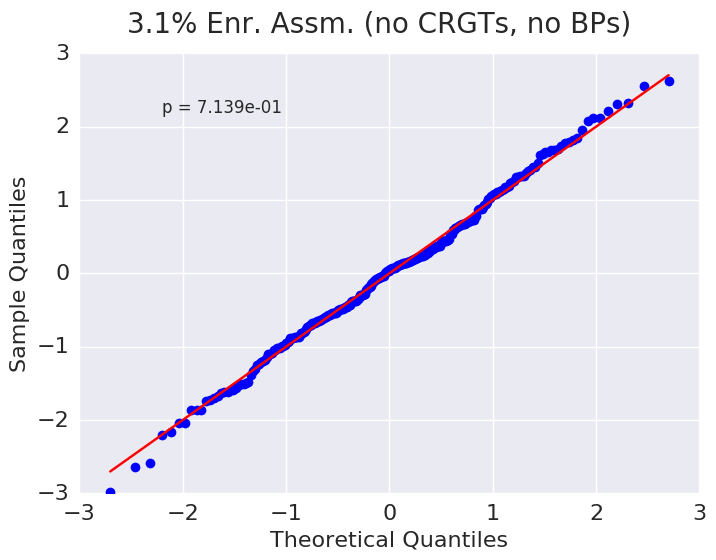
\includegraphics[width=\linewidth]{figures/patterns/assm-3.1-inf/quantile/assm-31-inf-capt-1}
  \caption{}
  \label{fig:chap9-qq-assm-3.1-inf-capt}
\end{subfigure}%
\begin{subfigure}{0.5\textwidth}
  \centering
  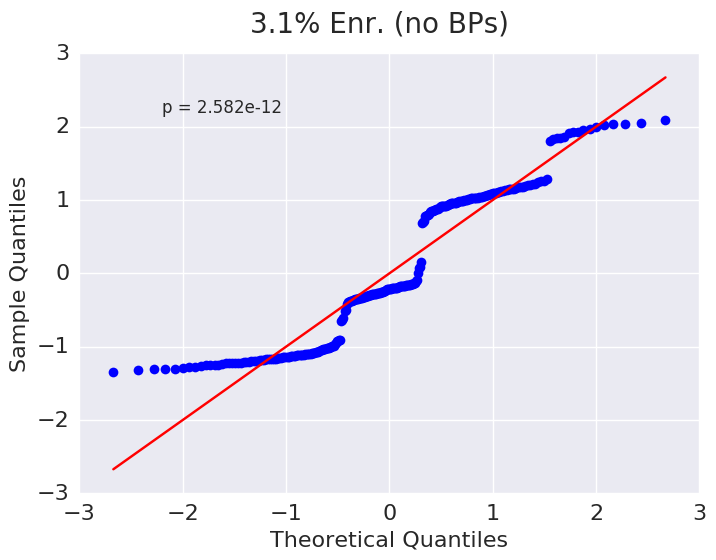
\includegraphics[width=\linewidth]{figures/patterns/assm-3.1/quantile/assm-31-capt-1}
  \caption{}
  \label{fig:chap9-qq-assm-3.1-capt}
\end{subfigure}
\begin{subfigure}{0.5\textwidth}
  \centering
  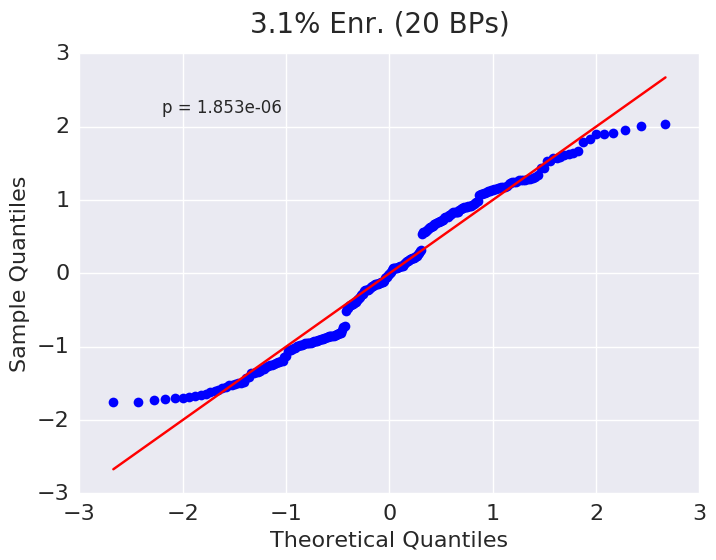
\includegraphics[width=\linewidth]{figures/patterns/assm-3.1-20BPs/quantile/assm-31-20BPs-capt-1}
  \caption{}
  \label{fig:chap9-qq-assm-3.1-20BPs-capt}
\end{subfigure}%
\begin{subfigure}{0.5\textwidth}
  \centering
  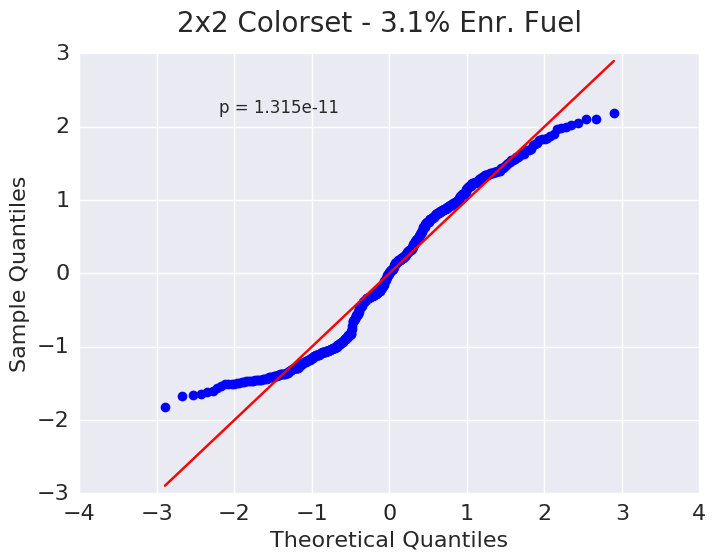
\includegraphics[width=\linewidth]{figures/patterns/2x2/quantile/31-enr-capt-1}
  \caption{}
  \label{fig:chap9-qq-2x2-3.1-capt}
\end{subfigure}
\begin{subfigure}{0.5\textwidth}
  \centering
  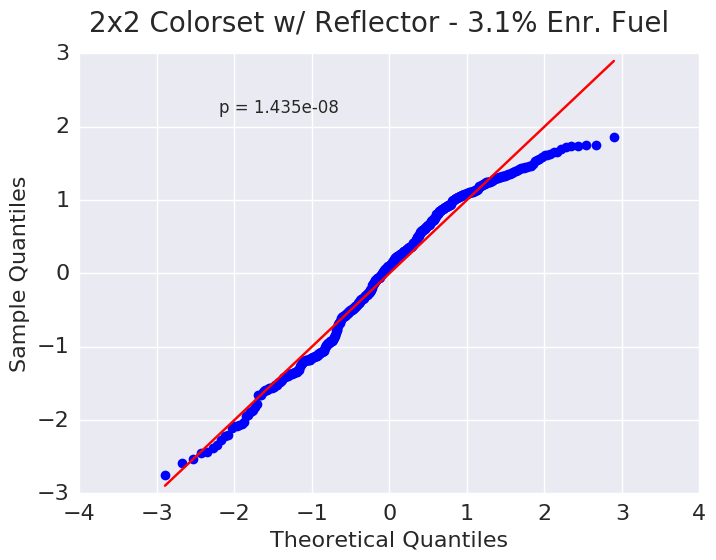
\includegraphics[width=\linewidth]{figures/patterns/reflector/quantile/31-enr-capt-1}  \caption{}
  \label{fig:chap9-qq-reflector-3.1-capt}
\end{subfigure}%
\begin{subfigure}{0.5\textwidth}
  \centering
  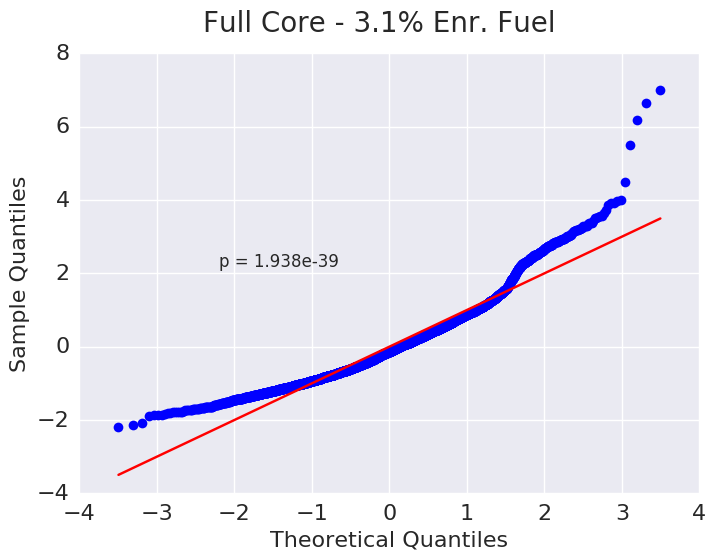
\includegraphics[width=\linewidth]{figures/patterns/full-core/quantile/31-enr-capt-1} \caption{}
  \label{fig:chap9-qq-full-core-3.1-capt}
\end{subfigure}
\caption[Q-Q plots of U-238 capture MGXS for 3.1\% enriched fuel]{Q-Q plots of U-238 capture \ac{MGXS} for 3.1\% enriched fuel.}
\label{fig:chap9-qq-3.1-capt}
\end{figure}

%%%%%%%%%%%%%%%%%%%%%%%%%%%%%%%%%%
\subsubsection{U-235 Fission MGXS}
\label{subsubsec:chap9-qq-plots-fiss}

first paragraph: intro U-235 fission \ac{MGXS} qq plots
-Fig.~\ref{fig:chap9-qq-1.6-fiss} and ~\ref{fig:chap9-qq-3.1-fiss}
  -U-235 fission \ac{MGXS} for 1.6\% and 3.1\% enriched fuel pins
  -in each of the heterogeneous benchmarks, respectively
-recall the inf. lattice case

-second paragraph:
  -the qq plot shows that data for the inf. lattices very nearly normal (p-values well above 0.05, closer to 0.35)
  -clear deviation from normality with addition of \acp{CRGT}
    -more complicated and less distinct structure than was seen for U-238 capture
  -crazy piecewise step-like structure with addition of \acp{BP}
    -much more fragmented than for U-238 capture
  -colorsets indicate sharper steps than for U-238 capture which ``smoothed'' out with more complexity
  -p-value is very clearly smallest for the full core (1e-22 and 1e-39 for 1.6\% and 3.1\% enr fuel)

-mention that tails above and below on lower/upper range indicate that tails of distribution are not as wide as would be expected for normal samples -- e.g., a ``tighter'' or ``narrower'' distribution
-3.1\% enr pins in full core are tighter on bottom edge, but wider on upper edge
  -indicative of those few ``outlier'' pins with \ac{MGXS} near 0.9 barns in Fig.~\ref{fig:chap9-hist-3.1-capt}

SUMMARY BOX

-what are key differences with U-238 capture plots?
-add ``Assm.'' to titles of plots for individual fuel assemblies
-add group 1/2 to captions

\begin{figure}[h!]
\centering
\begin{subfigure}{0.5\textwidth}
  \centering
  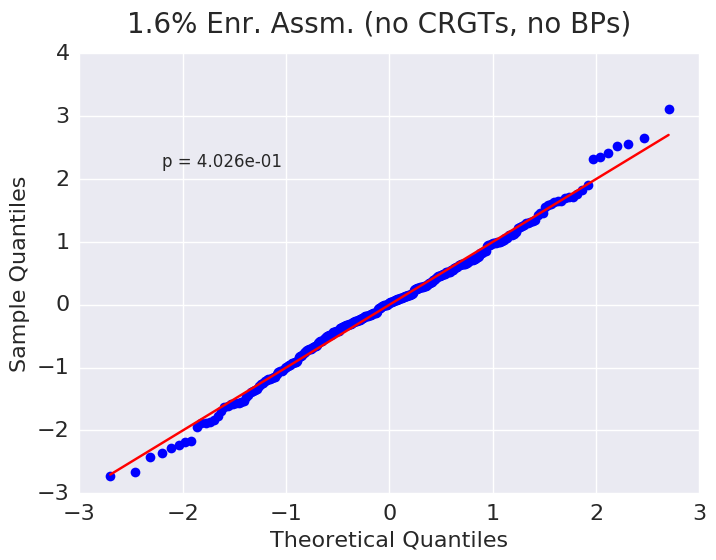
\includegraphics[width=\linewidth]{figures/patterns/assm-1.6-inf/quantile/assm-16-inf-fiss-2}
  \caption{}
  \label{fig:chap9-qq-assm-1.6-inf-fiss}
\end{subfigure}%
\begin{subfigure}{0.5\textwidth}
  \centering
  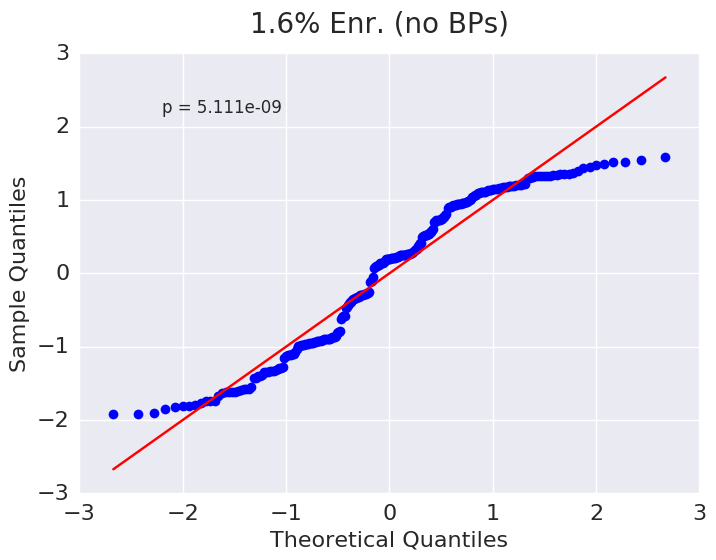
\includegraphics[width=\linewidth]{figures/patterns/assm-1.6/quantile/assm-16-fiss-2}
  \caption{}
  \label{fig:chap9-qq-assm-1.6-fiss}
\end{subfigure}
\begin{subfigure}{0.5\textwidth}
  \centering
  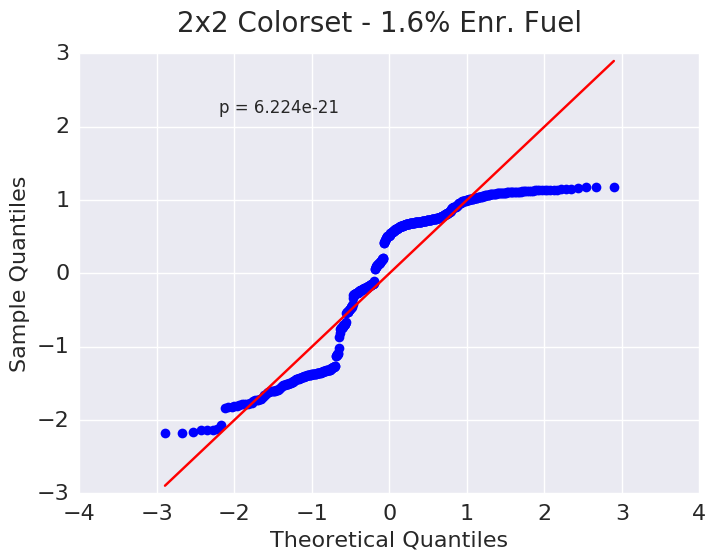
\includegraphics[width=\linewidth]{figures/patterns/2x2/quantile/16-enr-fiss-2}
  \caption{}
  \label{fig:chap9-qq-2x2-1.6-fiss}
\end{subfigure}%
\begin{subfigure}{0.5\textwidth}
  \centering
  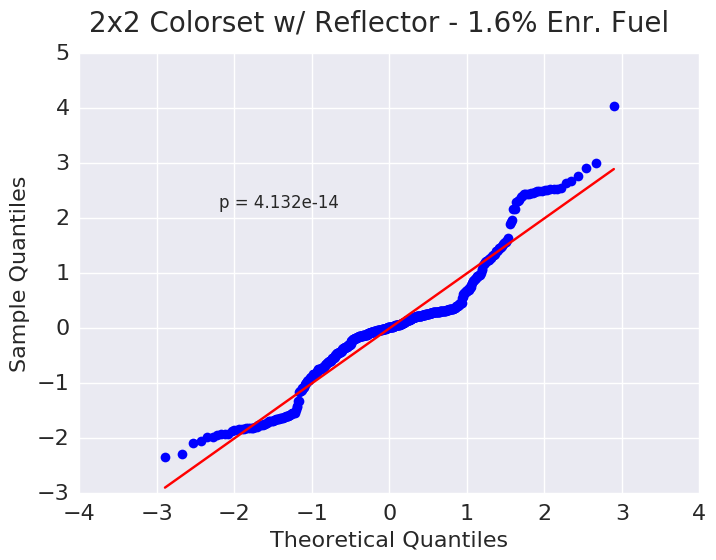
\includegraphics[width=\linewidth]{figures/patterns/reflector/quantile/16-enr-fiss-2}  \caption{}
  \label{fig:chap9-qq-reflector-1.6-fiss}
\end{subfigure}
\begin{subfigure}{0.5\textwidth}
  \centering
  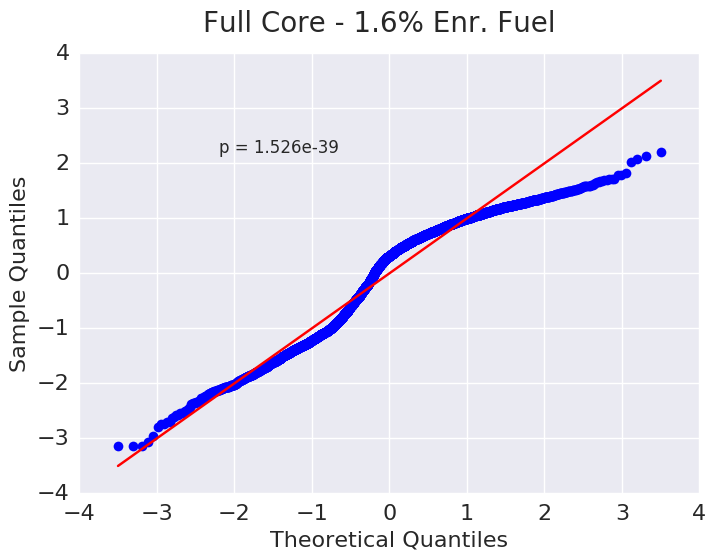
\includegraphics[width=\linewidth]{figures/patterns/full-core/quantile/16-enr-fiss-2} \caption{}
  \label{fig:chap9-qq-full-core-1.6-fiss}
\end{subfigure}
\caption[Q-Q plots of U-235 fission MGXS for 1.6\% enriched fuel]{Q-Q plots of U-235 fission \ac{MGXS} for 1.6\% enriched fuel.}
\label{fig:chap9-qq-1.6-fiss}
\end{figure}

\begin{figure}[h!]
\centering
\begin{subfigure}{0.5\textwidth}
  \centering
  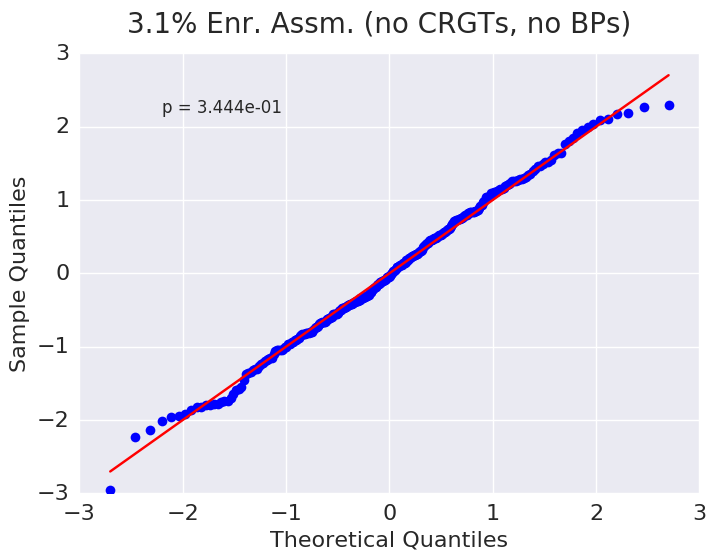
\includegraphics[width=\linewidth]{figures/patterns/assm-3.1-inf/quantile/assm-31-inf-fiss-2}
  \caption{}
  \label{fig:chap9-qq-assm-3.1-inf-fiss}
\end{subfigure}%
\begin{subfigure}{0.5\textwidth}
  \centering
  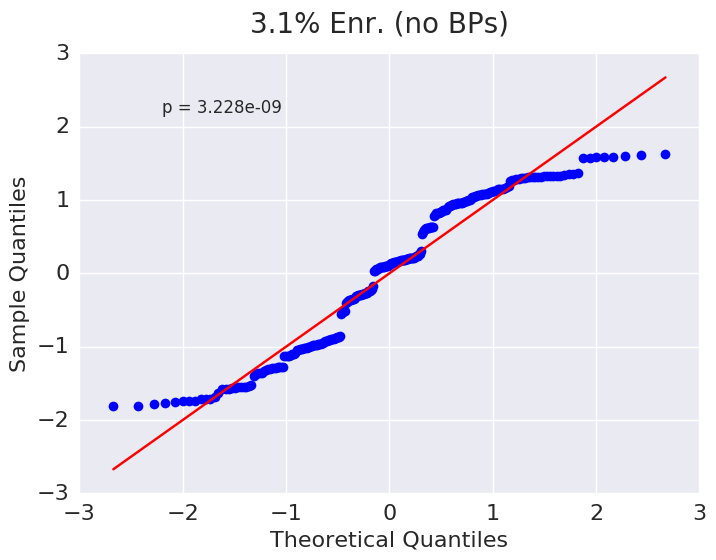
\includegraphics[width=\linewidth]{figures/patterns/assm-3.1/quantile/assm-31-fiss-2}
  \caption{}
  \label{fig:chap9-qq-assm-3.1-fiss}
\end{subfigure}
\begin{subfigure}{0.5\textwidth}
  \centering
  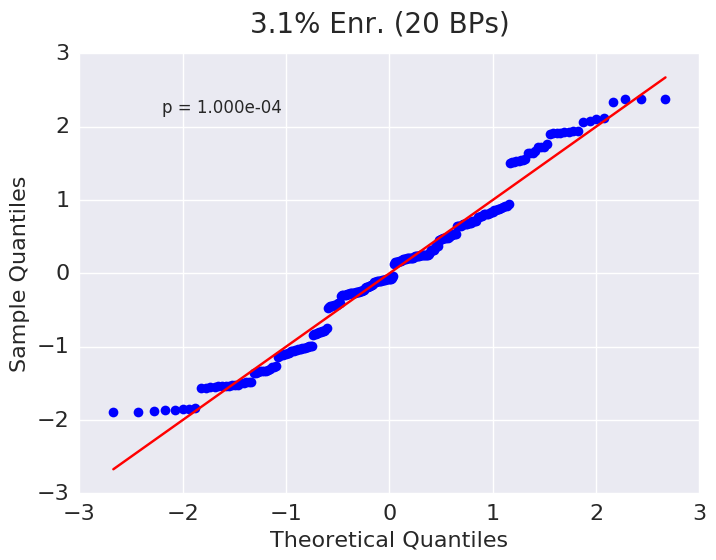
\includegraphics[width=\linewidth]{figures/patterns/assm-3.1-20BPs/quantile/assm-31-20BPs-fiss-2}
  \caption{}
  \label{fig:chap9-qq-assm-3.1-20BPs-fiss}
\end{subfigure}%
\begin{subfigure}{0.5\textwidth}
  \centering
  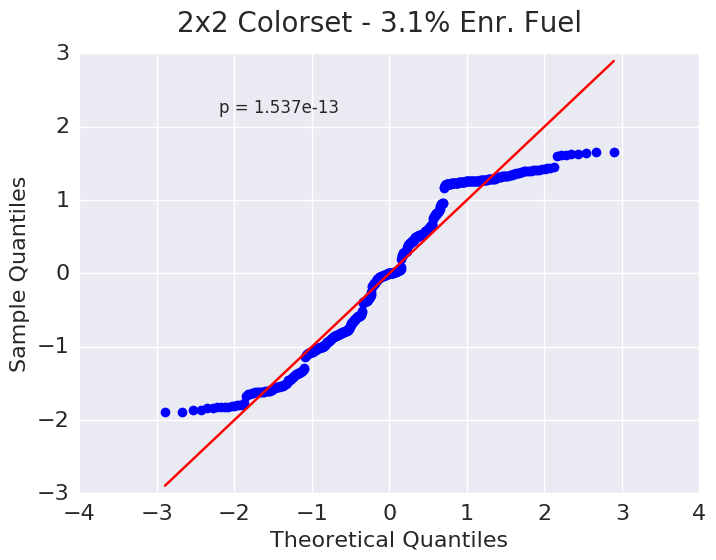
\includegraphics[width=\linewidth]{figures/patterns/2x2/quantile/31-enr-fiss-2}
  \caption{}
  \label{fig:chap9-qq-2x2-3.1-fiss}
\end{subfigure}
\begin{subfigure}{0.5\textwidth}
  \centering
  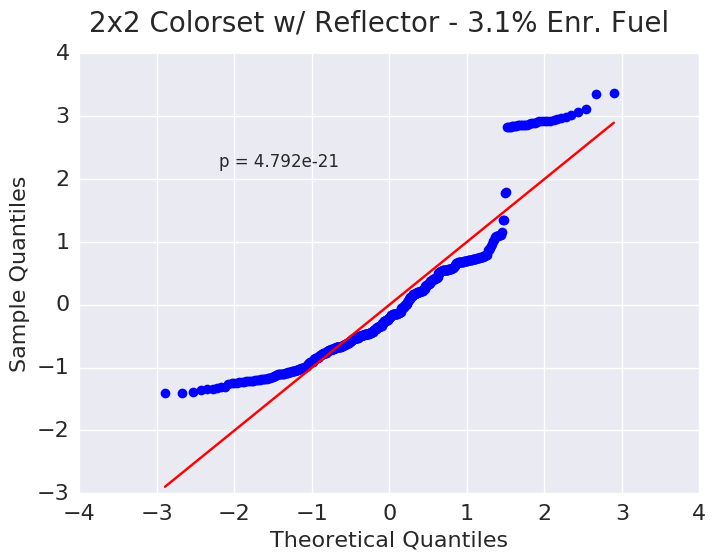
\includegraphics[width=\linewidth]{figures/patterns/reflector/quantile/31-enr-fiss-2}  \caption{}
  \label{fig:chap9-qq-reflector-3.1-fiss}
\end{subfigure}%
\begin{subfigure}{0.5\textwidth}
  \centering
  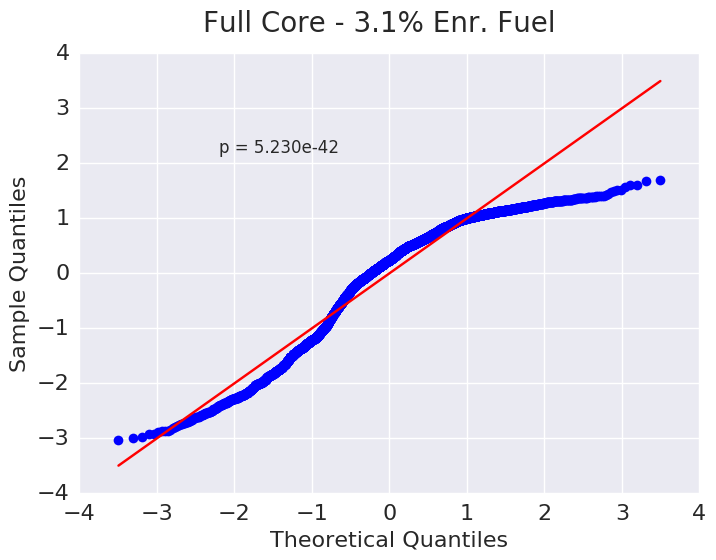
\includegraphics[width=\linewidth]{figures/patterns/full-core/quantile/31-enr-fiss-2} \caption{}
  \label{fig:chap9-qq-full-core-3.1-fiss}
\end{subfigure}
\caption[Q-Q plots of U-235 fission MGXS 3.1\% enriched fuel]{Q-Q plots of U-235 fission \ac{MGXS} for 3.1\% enriched fuel.}
\label{fig:chap9-qq-3.1-fiss}
\end{figure}


%%%%%%%%%%%%%%%%%%%%%%%%%%%%%%%%%%%%%%%%%%%%%%%%%%%%%%%%%%%%%%%%%%%%%%%%%%%%%%%
\section{LNS Spatial Homogenization}
\label{sec:chap9-lns-homogenize}

first paragraph: 
-recall geometric templates used in traditional lattice physics codes
  -CASMO~\cite{rhodes2006casmo}
-recall OpenCG's \ac{LNS} algorithm from Sec.~\ref{sec:chap4-lns}
  -used as a proxy for geometric templates
-this section applies it as a deterministic atttempt to ``cluster'' like \ac{MGXS}
-aim is to predict U-238 capture rates better than is possible with null/infinite homogenization
  -approach degenerate homogenization's accuracy
  -accelerate tally convergence rate by averaging \ac{MGXS} across many pin instances
    -refer to last section of this chapter

second paragraph: describe \ac{LNS} spatial homogenization
-tally \ac{MGXS} for each fuel pin instance across the core
  -as is done for degenerate homogenization
-use OpenCG \ac{LNS} algorithm to assign an \ac{LNS} identifier to each unique pin instance in \ac{CG}
  -pins with like neighboring pins will receive the same \ac{LNS} identifier
-average \ac{MGXS} for each ``family'' of pin instances with like \ac{LNS} identifiers
  -mention what this means - sum up flux and reaction rate tallies
    -effectively an average weighted by track density in each pin
    -equivalent to defining flux/rxn rate tallies specifically for those fuel pin intances
    -perhaps use an equation for this???
-\ac{MGXS} for all other materials are averaged across the complete heterogeneous geometry
  -take wording from last chapter for this

third paragraph: point out materials for the six benchmarks
-Tab.~\ref{table:chap9-num-materials-lns} 
  -number of materials for each of the six benchmarks with \ac{LNS} homogenization
-Fig.~\ref{fig:chap9-lns-materials}
  -materials configurations for individual assembly and 2$\times$2 colorset benchmarks with \ac{LNS} spatial homogenization
-Fig.~\ref{fig:chap9-lns-materials-beavrs}
  -materials configuration for 2D quarter core \ac{BEAVRS} model with \ac{LNS} spatial homogenization

fourth paragraph: segue to next chapter
-objective is to capture clustering effects in MGXS
-LNS isn't adaptable
  -point out pins along assembly-assembly and assembly-reflector interfaces treated the same
  -point out large number of materials in full core - may be more than necessary
  -algorithm must be customized to specific types of core geometries
-following section will highlight the results with \ac{LNS} spatial homogenization

\begin{table}[h!]
  \centering
  \caption[Number of materials for LNS spatial homogenization]{Number of materials modeled with unique \ac{MGXS} in each heterogeneous benchmark for \ac{LNS} spatial homogenization.}
  \small
  \label{table:chap9-num-materials-lns}
  \vspace{6pt}
  \begin{tabular}{l r r r}
  \toprule
  \rowcolor{lightgray}
  & \multicolumn{3}{c}{\cellcolor{lightgray} \bf \# Materials} \\
  \multirow{-2}{*}{\cellcolor{lightgray} \bf Benchmark} &
  \multicolumn{1}{c}{\cellcolor{lightgray} \bf Null/Infinite} &
  \multicolumn{1}{c}{\cellcolor{lightgray} \bf \ac{LNS}} &
  \multicolumn{1}{c}{\cellcolor{lightgray} \bf Degenerate} \\
  \midrule
1.6\% Assm & 5 & 13 & 268 \\
  \midrule
3.1\% Assm & 5 & 13 & 268 \\
  \midrule
3.1\% Assm w/ 20 BPs & 7 & 17 & 270  \\
  \midrule
2$\times$2 Colorset & 8 & 25 & 1,062 \\
  \midrule
2$\times$2 Colorset w/ Reflector & 8 & 35 & 1,062 \\
  \midrule
\ac{BEAVRS} Quarter Core & 10 & 497 & 13,000 \\ % LNS = ceil(193 / 4) * 10 + 7
  \bottomrule
\end{tabular}
\end{table}

\begin{figure}[h!]
\centering
\begin{subfigure}{.47\textwidth}
  \centering
  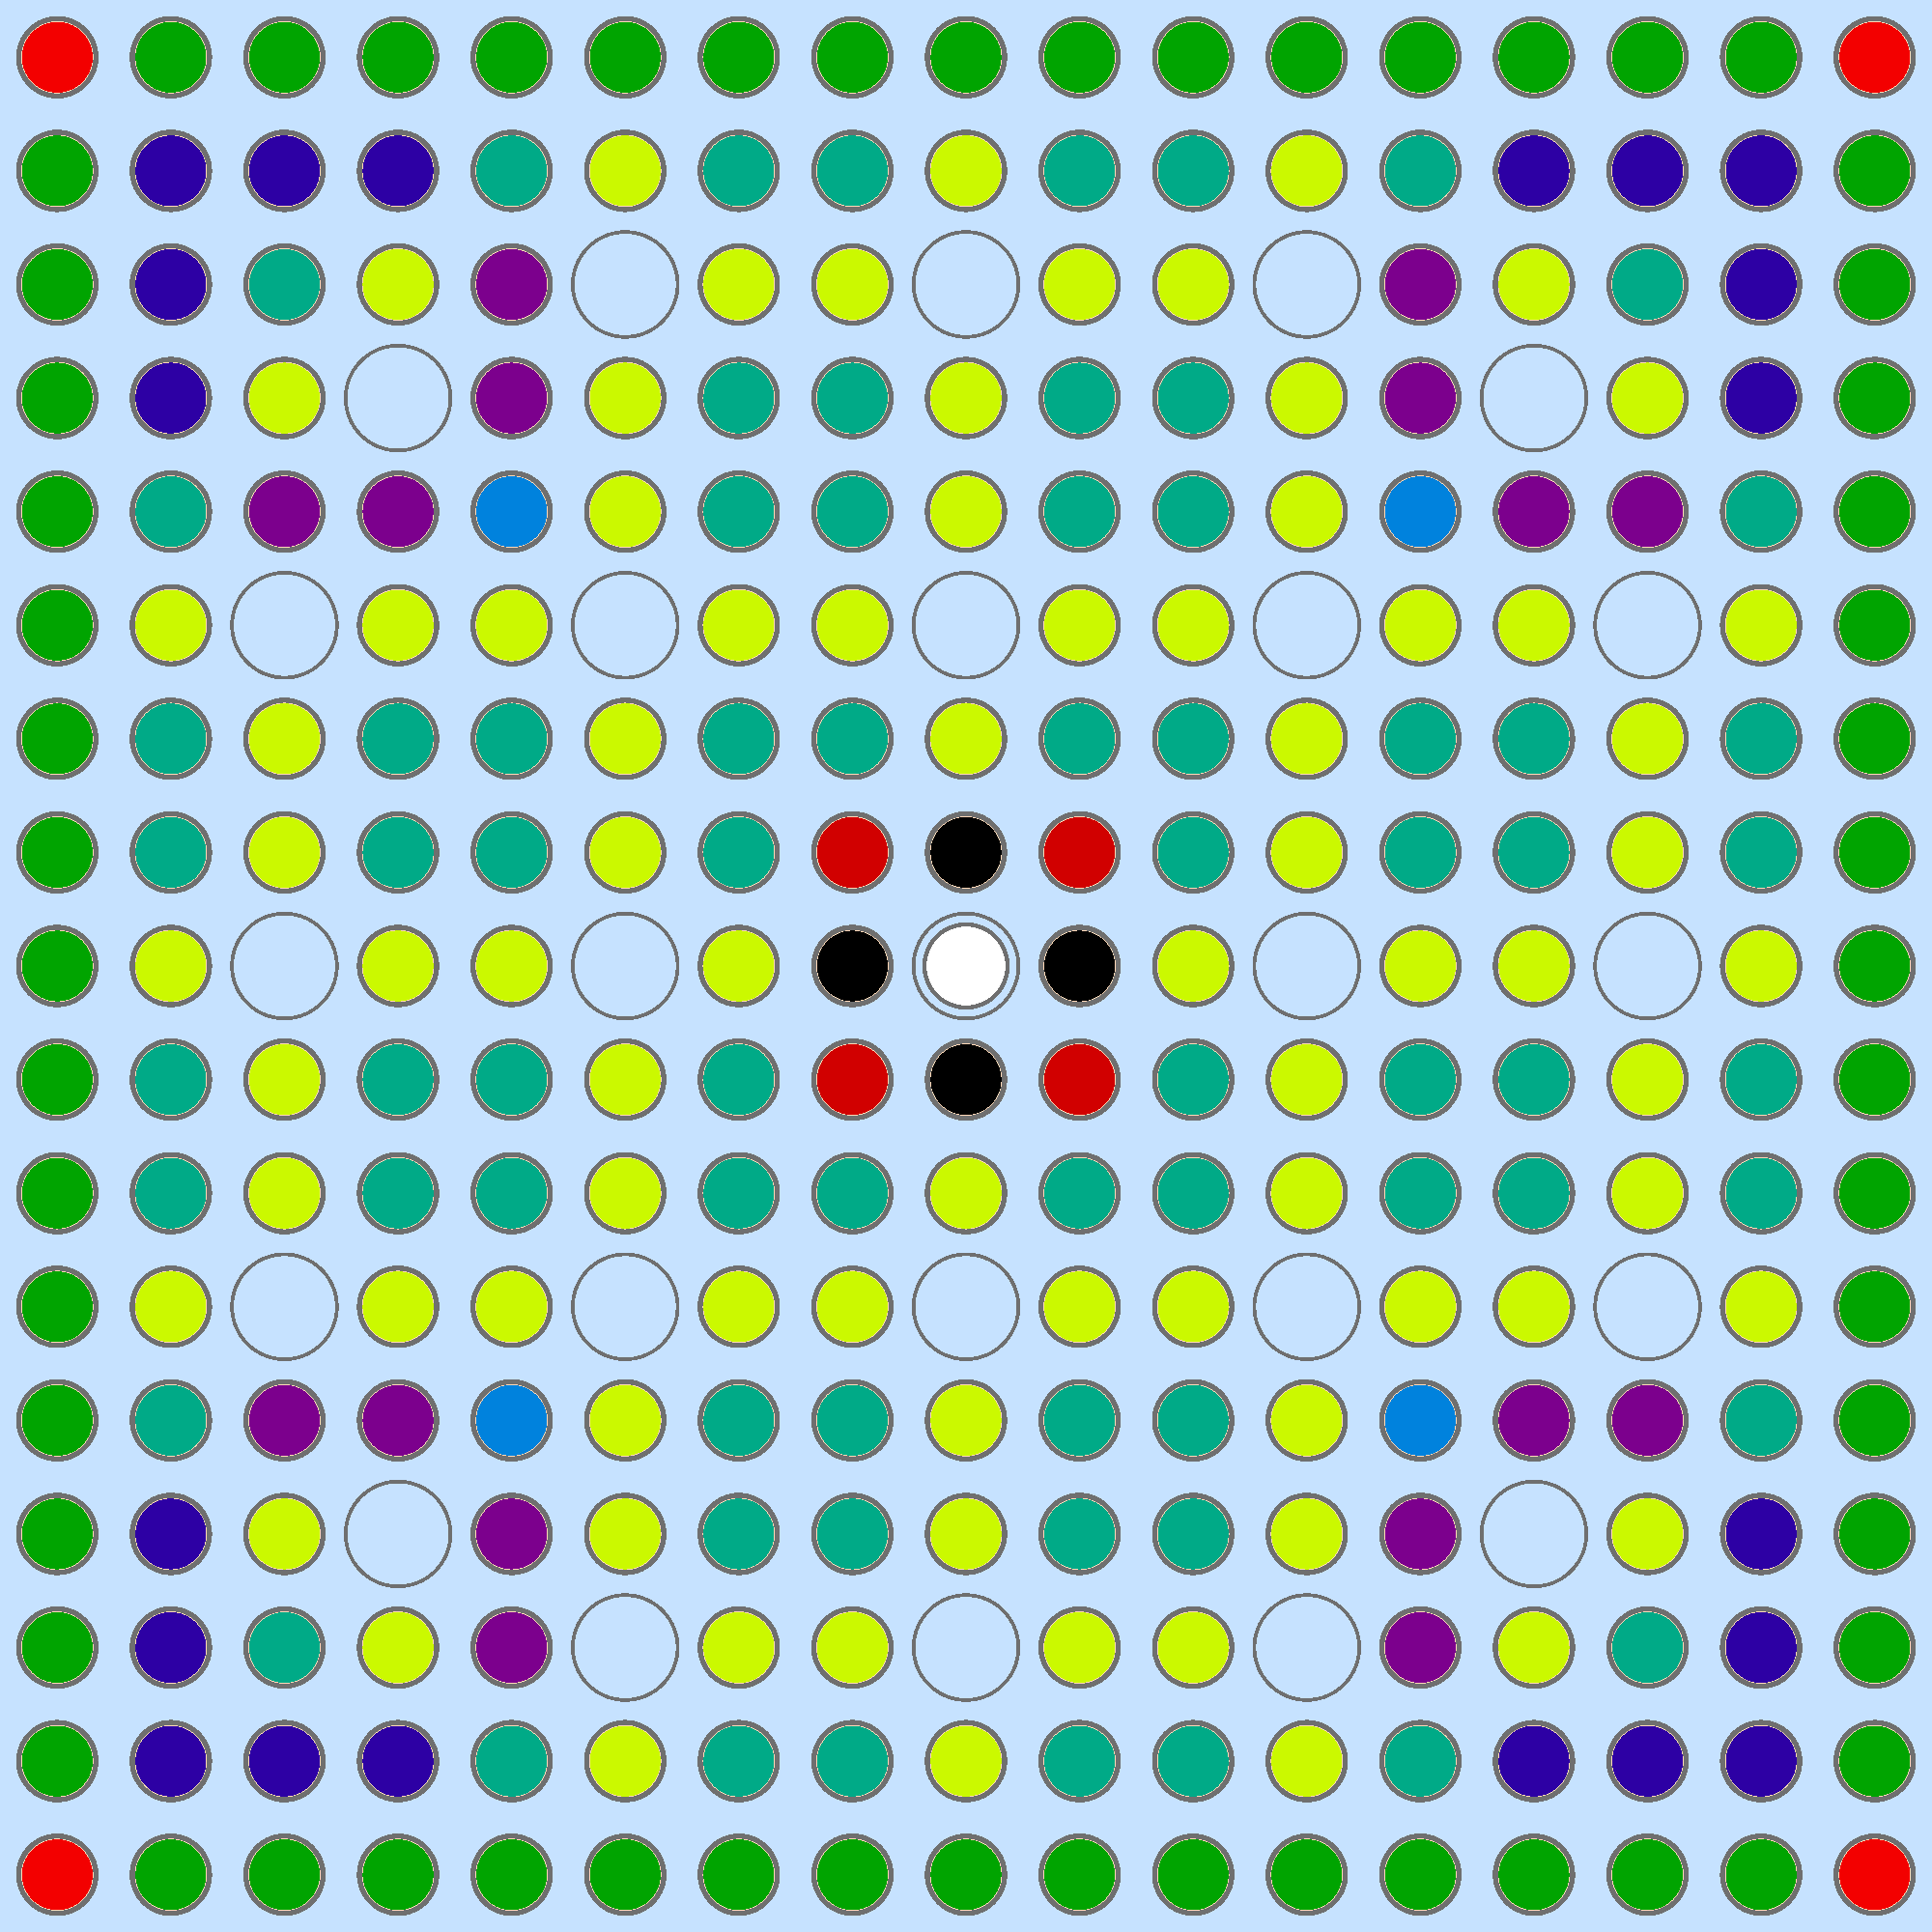
\includegraphics[width=0.9\linewidth]{figures/patterns/lns/assm-31/materials}
  \caption{}
  \label{fig:chap9-assm-31-lns-materials}
\end{subfigure}%
\begin{subfigure}{.47\textwidth}
  \centering
  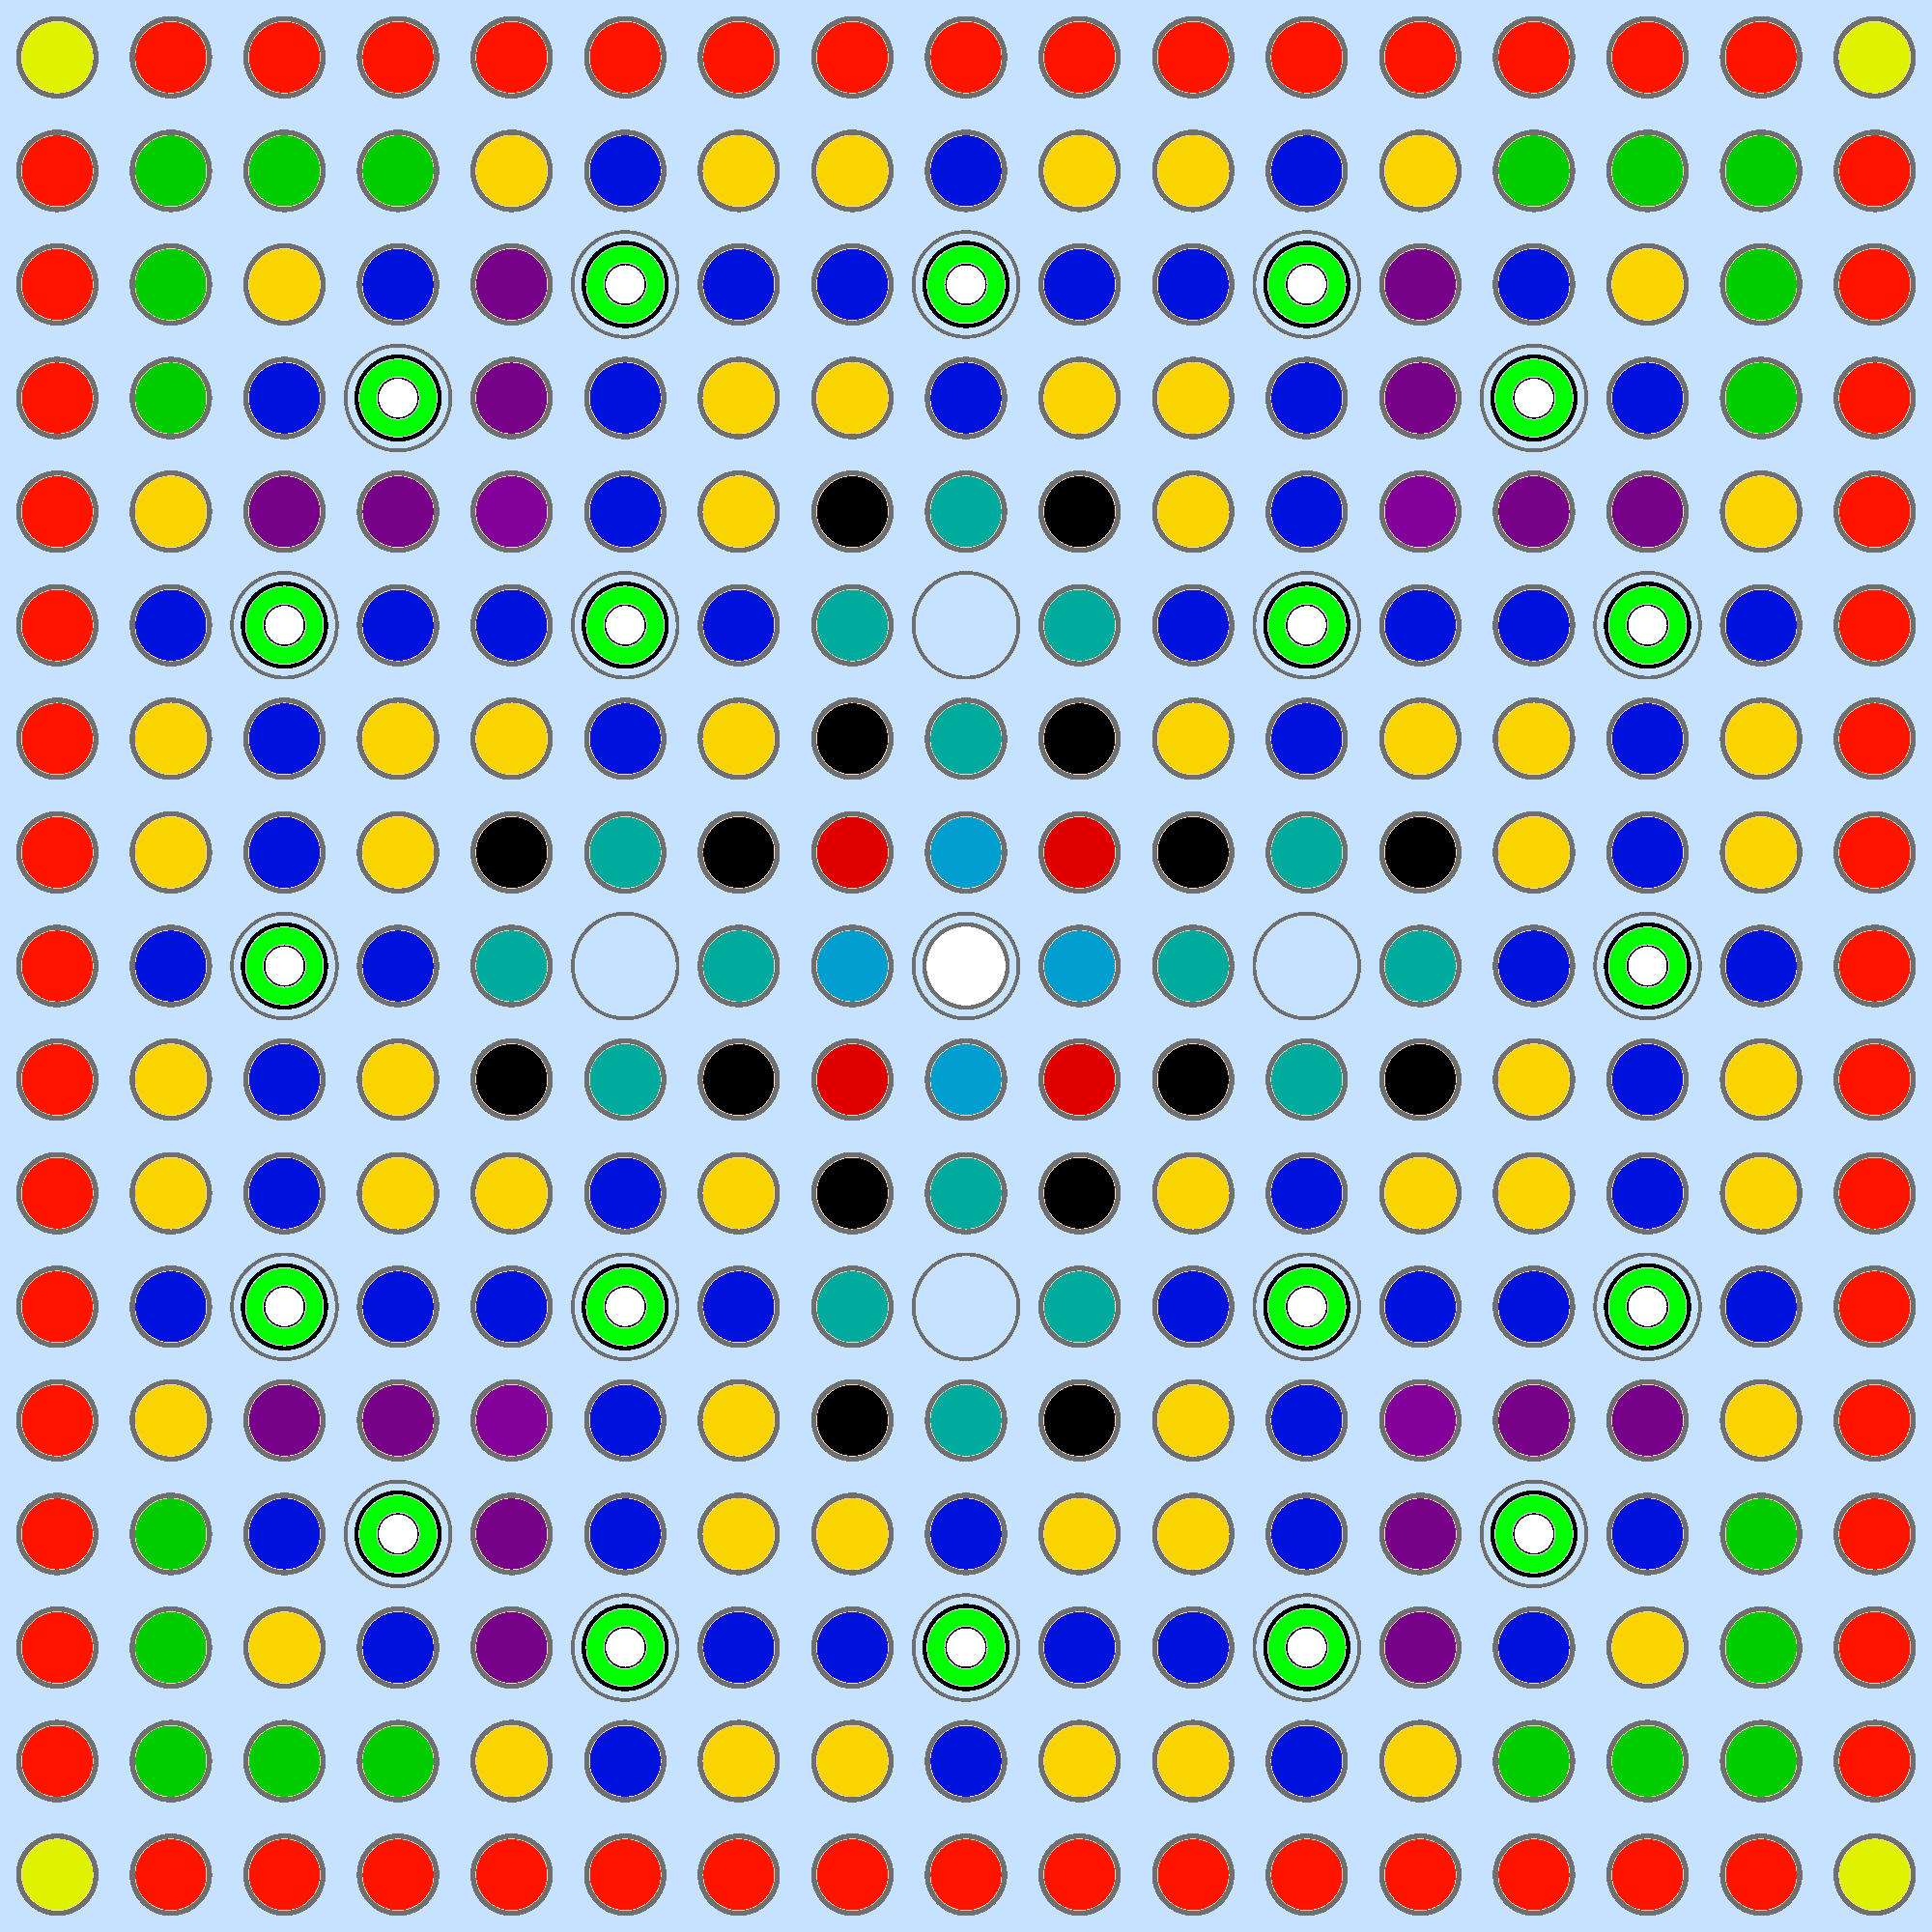
\includegraphics[width=0.9\linewidth]{figures/patterns/lns/assm-31-20BPs/materials}
  \caption{}
  \label{fig:chap9-31-20BPs-lns-materials}
\end{subfigure}
\begin{subfigure}{.47\textwidth}
  \centering
  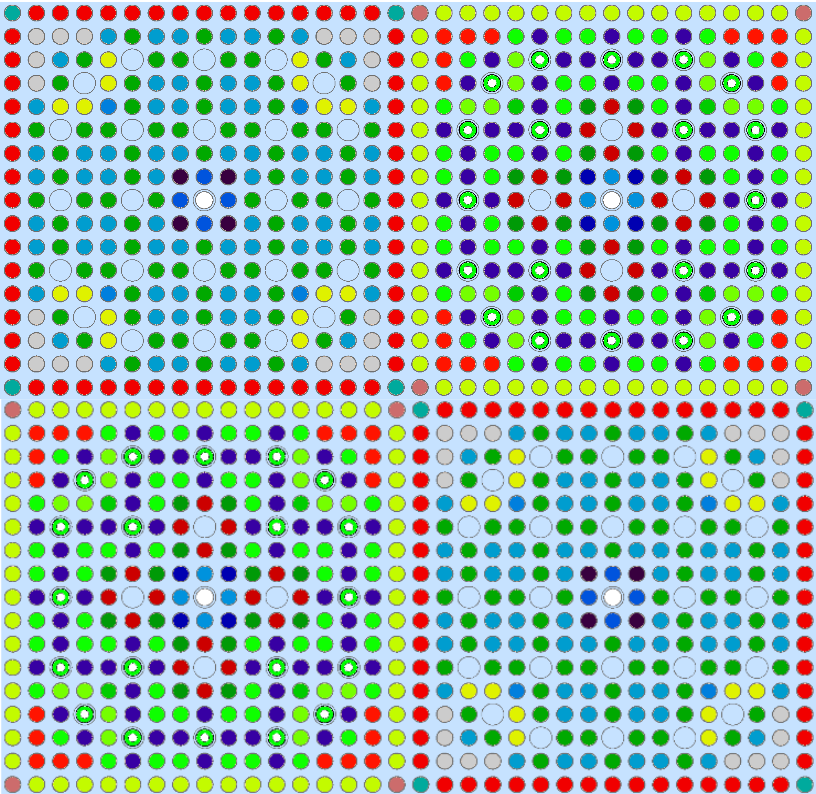
\includegraphics[width=0.9\linewidth]{figures/patterns/lns/2x2/materials}
  \caption{}
  \label{fig:chap9-2x2-lns-materials}
\end{subfigure}%
\begin{subfigure}{.47\textwidth}
  \centering
  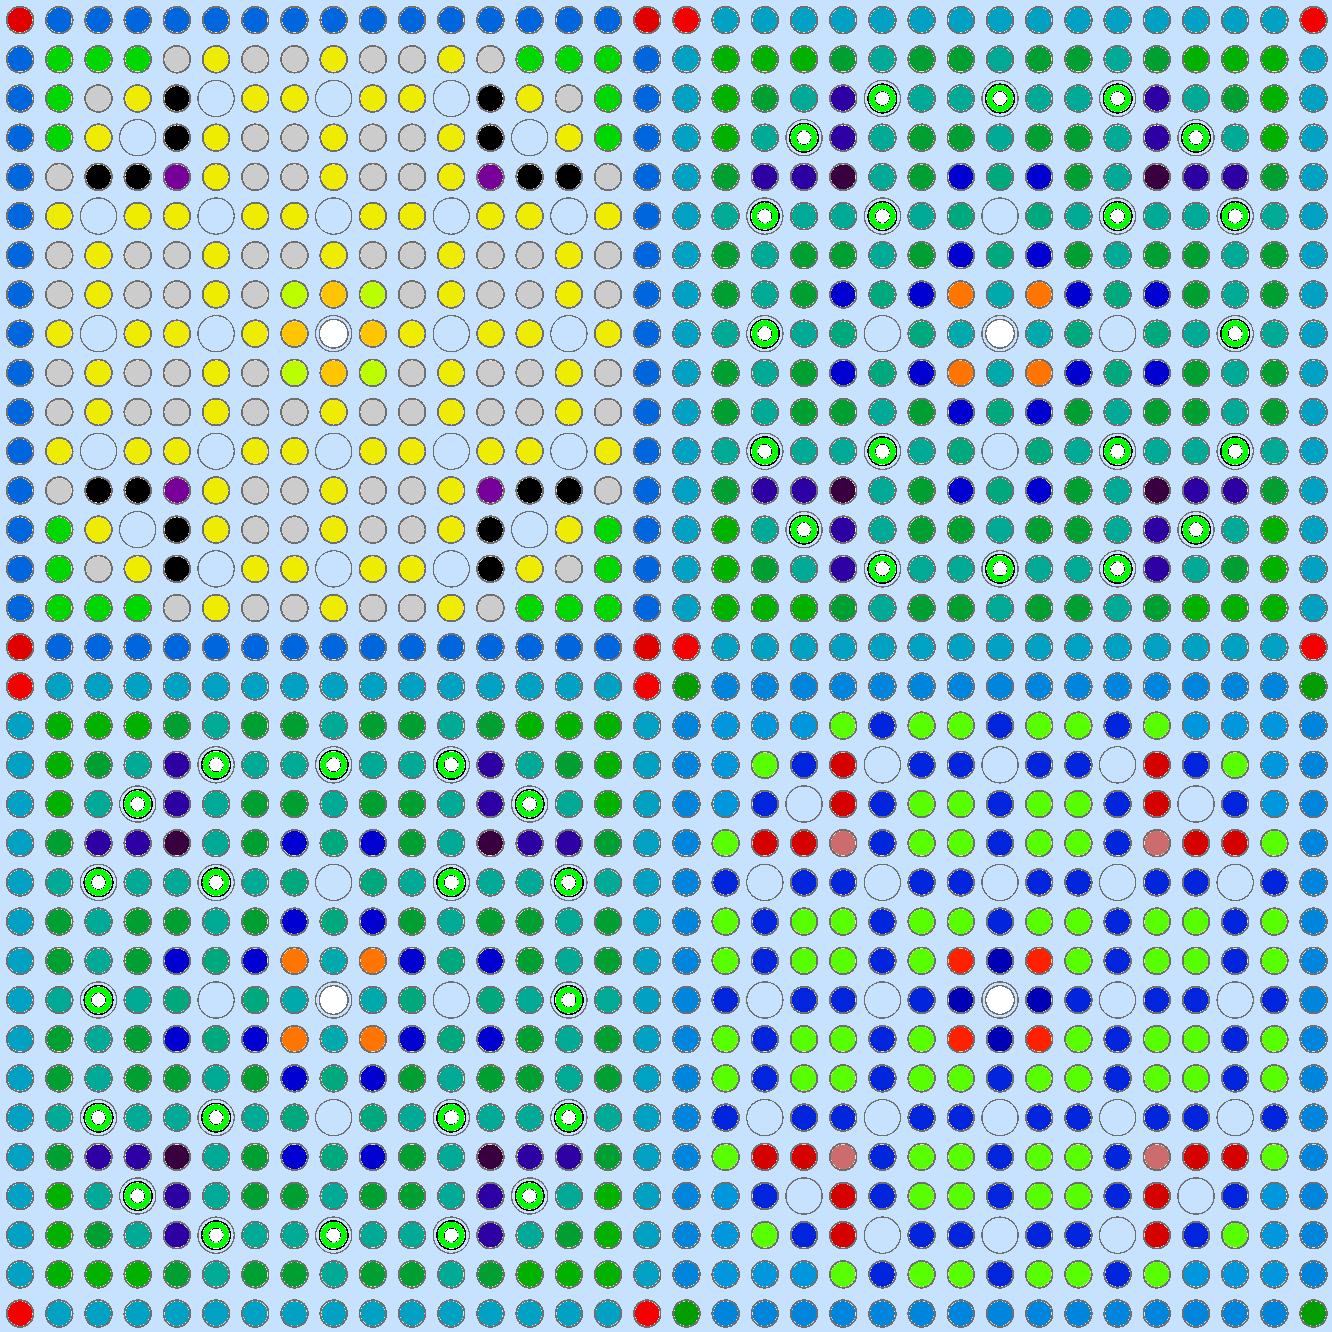
\includegraphics[width=0.9\linewidth]{figures/patterns/lns/reflector/materials}
  \caption{}
  \label{fig:chap9-reflector-lns-materials}
\end{subfigure}
\caption[Depiction of LNS spatially homogenized materials]{OpenMOC materials with \ac{LNS} spatial homogenization for a 1.6/3.1\% enriched fuel assembly (a), a 3.1\% enriched assembly with 20 \acp{BP} (b), a 2$\times$2 colorset without (c) and with (d) a reflector. Each uniquely colored material represents a unique set of \ac{MGXS}.}
\label{fig:chap9-lns-materials}
\end{figure}

\begin{figure}[h!]
\centering
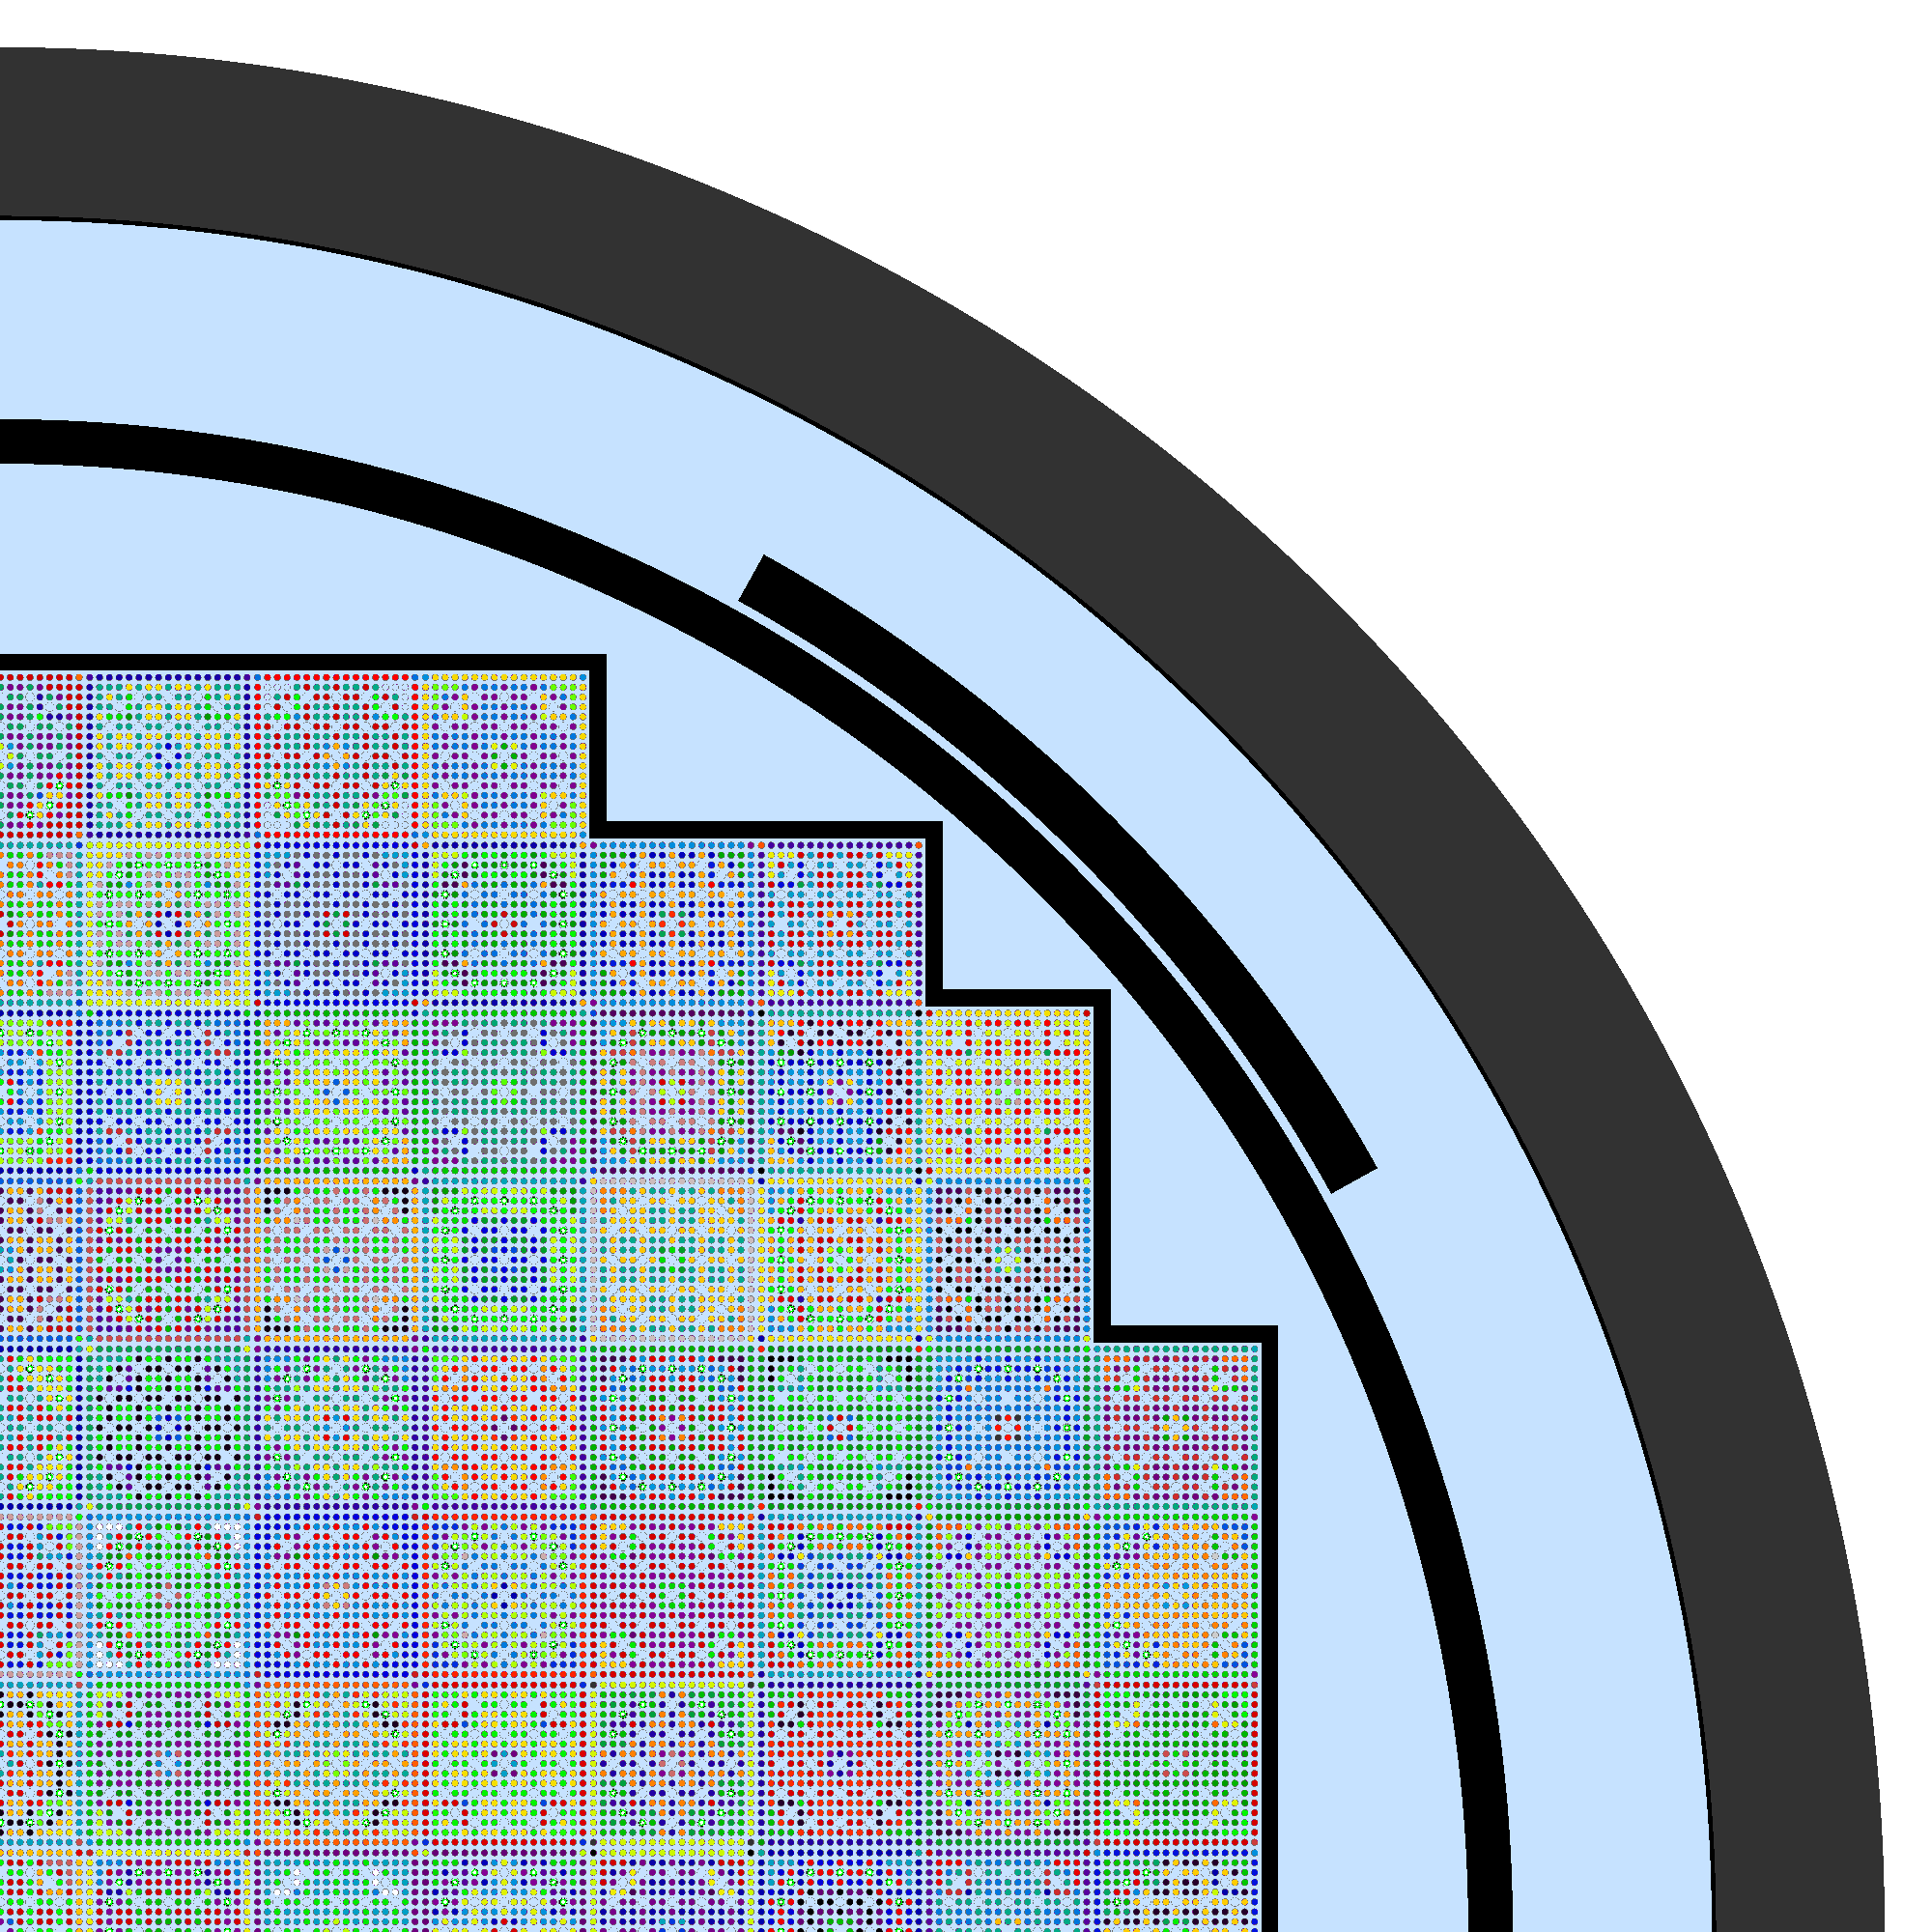
\includegraphics[width=\linewidth]{figures/patterns/lns/full-core/materials}
\caption{}
\caption[Depiction of LNS spatially homogenized materials for quarter core BEAVRS]{OpenMOC materials with \ac{LNS} spatial homogenization for the 2D quarter core \ac{BEAVRS} model. Each uniquely colored material represents a unique set of \ac{MGXS}.}
\label{fig:chap9-lns-materials-beavrs}
\end{figure}


%%%%%%%%%%%%%%%%%%%%%%%%%%%%%%%%%%%%%%%%%%%%%%%%%%%%%%%%%%%%%%%%%%%%%%%%%%%%%%%%
\section{Multi-Group Results with LNS}
\label{subsec:chap9-lns-results}

first paragraph: introduce / outline results
-ran simulations with 2, 8 and 70 groups as in Chap.~\ref{chap:quantify} for each of the six benchmarks
-used \ac{LNS} spatial homogenization in each one with same OpenMOC simulation parameters
  -128 azimuthal angles, 0.05 cm track spacing
-Sec.~\ref{subsec:chap9-lns-eigenvalues} - eigenvalues
-Sec.~\ref{subsec:chap9-lns-fiss-rates} - pin-wise energy-integrated fission rates
-Sec.~\ref{subsec:chap9-lns-capt-rates} - pin-wise energy-integrated capture rates

%%%%%%%%%%%%%%%%%%%%%%%%
\subsection{Eigenvalues}
\label{subsec:chap9-lns-eigenvalues}

first paragraph: eigenvalues
-as was observed when comparing null to degenerate homogenization in Chap.~\ref{chap:quantify}, spatial homogenization cannot be expected to systematically improve the eigenvalue wrt OpenMC
-but these results are presented here to ensure that \ac{LNS} homogenization was properly implemented
  -and results simply reinforce this notion
-Tab.~\ref{table:chap9-lns-eigenvalues} tabulates eigenvalues for 2, 8, and 70 groups
-eigenvalues closely match null and degenerate homogenization from Chap.~\ref{chap:quantify}
  -match to within less than 10 \ac{pcm} for nearly all cases
  -due to reaction rate preservation

\begin{table}[ht!]
  \centering
  \caption[OpenMOC eigenvalue bias with LNS homogenization]{OpenMOC eigenvalue bias $\Delta\rho$ for heterogeneous benchmarks with \ac{LNS} homogenization and varying energy group structures.}
  \small
  \label{table:chap9-lns-eigenvalues}
  \vspace{6pt}
  \begin{tabular}{l R{2.5cm} R{2.5cm} R{2.5cm}}
  \toprule
  \rowcolor{lightgray}
  & \multicolumn{3}{S[table-format=6.1]}{\cellcolor{lightgray} {$\bm{\Delta\rho}$ \textbf{[pcm]}}} \\
  \multirow{-2}{*}{\cellcolor{lightgray} \bf Benchmark} &
  \multicolumn{1}{r}{{\cellcolor{lightgray} \bf 2-Group}} &
  \multicolumn{1}{r}{{\cellcolor{lightgray} \bf 8-Group}} &
  \multicolumn{1}{r}{{\cellcolor{lightgray} \bf 70-Group}} \\
  \midrule
1.6\% Assm & 56 & -79 & -168 \\
3.1\% Assm & 97 & -80 & -202 \\
3.1\% Assm w/ 20 BPs & -157 & -161 & -247 \\
2$\times$2 Colorset & 10 & -94 & -195 \\
2$\times$2 Colorset w/ Reflector & 1792 & 476 & -143 \\
BEAVRS Full Core & 2225 & 448 & -81 \\
  \bottomrule
\end{tabular}
\end{table}

%%%%%%%%%%%%%%%%%%%%%%%%
\subsection{Fission Rates}
\label{subsec:chap9-lns-fiss-rates}

first paragraph: overview of error trends
-Tab.~\ref{table:chap9-lns-fiss-rates} - max and mean fission rate errors
  -compare to Tabs.~\ref{table:chap8-openmoc-max-fiss-rates} and~\ref{table:chap8-openmoc-mean-fiss-rates}
  -recall that degenerate homogenization provided little improvement in fission rates
-max rates - observations
  -assm 1.6 - very nearly the same as degenerate
  -assm 3.1 - similar to degenerate (better than null)
  -assm 3.1 w/ BPs - slightly better than degenerate for 8 and 70 groups
  -2x2 - similar to degenerate, but they all perform the same for 70 groups
  -2x2 w/ reflector - significantly worse with 2 groups, and over 0.12\% worse than degenerate w/ 70 groups
  -largest deviation with degenerate is for 2 groups
-mean rates - observations
  -assm 1.6 - slightly better than degenerate for 8 and 70 groups (0.02\%)
  -assm 3.1 - slightly better than degenerate for 8 and 70 groups (0.02\%)
  -assm 3.1 w/ BPs - slightly better than degenerate for 70 groups (0.02\%)
  -2x2 - slightly better than degenerate for 8 and 70 groups (0.02\%)
  -2x2 w/ reflector - worse than degenerate, but better than null
-GENERAL TAKEWAWAY: generally better than null but approaches accuracy of degenerate case
  -except for reflector and full core
-depictions of spatial distributions of errors not shown here since it was shown in Chap.~\ref{chap:quantify} that spatial homogenization has little impact on fission rates

-SUMMARY BOX

\begin{table}[ht!]
  \centering
  \caption[OpenMOC fission rate errors with LNS homogenization]{OpenMOC fission rate percent relative errors for heterogeneous benchmarks with \ac{LNS} spatial homogenization and varying energy group structures.}
  \small
  \label{table:chap9-lns-fiss-rates}
  \vspace{6pt}
  \begin{tabular}{l l R{2.5cm} R{2.5cm} R{2.5cm}}
  \toprule
  \rowcolor{lightgray}
  & & \multicolumn{3}{c}{\cellcolor{lightgray} \textbf{Error [\%]}} \\
  \multirow{-2}{*}{\cellcolor{lightgray} \bf Benchmark} &
  \multirow{-2}{*}{\cellcolor{lightgray} \bf Metric} &
  \multicolumn{1}{r}{{\cellcolor{lightgray} \bf 2-Group}} &
  \multicolumn{1}{r}{{\cellcolor{lightgray} \bf 8-Group}} &
  \multicolumn{1}{r}{{\cellcolor{lightgray} \bf 70-Group}} \\
  \midrule
\multirow{2}{*}{\parbox{2.2cm}{1.6\% Assm}} & Max & 2.131 & 0.764 & 0.313 \\
& Mean & 0.714 & 0.239 & 0.083 \\
\midrule
\multirow{2}{*}{\parbox{2.2cm}{3.1\% Assm}} & Max & 2.476 & 0.919 & 0.429 \\
& Mean & 0.832 & 0.287 & 0.091 \\
\midrule
\multirow{2}{*}{\parbox{2.2cm}{3.1\% Assm w/ 20 BPs}} & Max & -2.009 & -0.715 & 0.369 \\
& Mean & 0.719 & 0.216 & 0.095 \\
\midrule
\multirow{2}{*}{\parbox{2.2cm}{2$\times$2 Colorset}} & Max & -5.517 & -1.490 & 0.584 \\
& Mean & 2.940 & 0.701 & 0.138 \\
\midrule
\multirow{2}{*}{\parbox{2.2cm}{2$\times$2 Colorset w/ Reflector}} & Max & -15.714 & -2.894 & 0.887 \\
& Mean & 5.170 & 1.076 & 0.178 \\
\midrule
\multirow{2}{*}{\parbox{2.2cm}{BEAVRS Full Core}} & Max & -86.166 & -35.548 & 12.330 \\
& Mean & 40.190 & 11.465 & 1.454 \\
\bottomrule
\end{tabular}
\end{table}

%%%%%%%%%%%%%%%%%%%%%%%%%%%%%%%%%%%%%%%%%%%%%
\subsection{U-238 Capture Rate Distributions}
\label{subsec:chap9-lns-capt-rates}

first paragraph:
-Tab.~\ref{table:chap9-lns-capt-rates} - max and mean U-238 capture rate errors
  -compare to Tabs.~\ref{table:chap8-openmoc-max-capt-rates} and~\ref{table:chap8-openmoc-mean-capt-rates}
  -recall that degenerate homogenization significantly reduced U-238 capture rate errors 
-max rates - observations
  -assm 1.6 - better than degenerate w/ 70 groups (0.04\%), but worse with 2 and 8 groups
  -assm 3.1 - better than degenerate w/ 70 groups (0.07\%), but worse with 2 and 8 groups
  -assm 3.1 w/ BPs - worse than degenerate w/ 70 groups (0.06\%)
  -2x2 - significantly better than degenerate w/ 70 groups (0.16\%)
  -2x2 w/ reflector - significantly worse than degenerate (and null) w/ 70 groups (0.8\%)
    -and with opposite sign since the errors are under-predicted near reflector
  -generally worse with 2 and 8 groups
-mean rates - observations
  -assm 1.6 - better than degenerate w/ 70 groups (0.01\%)
  -assm 3.1 - better than degenerate w/ 70 groups (0.01\%)
  -assm 3.1 w/ BPs - better than degenerate w/ 70 groups (0.01\%)
  -2x2 - better than degenerate w/ 70 groups (0.04\%)
  -2x2 w/ reflector - worse than degenerate w/ 70 groups (0.07\%)
    -though still much better than null/infinite
-GENERAL TAKEWAWAY: generally better than null but approaches accuracy of degenerate case
  -even slightly beats accuracy of degenerate case in most cases
  -except for reflector and full core

second paragraph: spatial distributions
-Figs.~\Crefrange{fig:chap9-assm-1.6-lns-capt-err}{fig:chap9-full-core-capt-err-degenerate}
  -U-238 capture rate error distributions with respect to OpenMC reference results
  -akin to Figs.~\Crefrange{fig:chap8-assm-1.6-capt-err}{fig:chap8-full-core-capt-err}
  -compare null, \ac{LNS} and degenerate homogenization for 8 and 70 groups
  -shows the error distributions for degenerate and \ac{LNS} spatial homogenization are very nearly the same for the individual fuel assemblies and 2$\times$2 colorset
  -error distributions deviate for the 2$\times$2 colorset with a reflector

third paragraph: observations with reflector?? w/ 70 groups
  -NULL
    -largest errors along assembly-assembly / assembly-reflector interfaces, and pins near \acp{CRGT}
  -DEGENERATE
    -errors randomly distributed across pins
  -LNS
    -largest errors along assembly-reflector interface, and lesser extent assembly-reflector interface
    -as shown in table, largest errors are larger than those for null case
    -reason is that LNS averages \ac{MGXS} pins along both interfaces rather than differentiating b/w them
    -this is actually a worse approx. than averaging across ALL pins as is done by null case
    -highlights sensitivity to how \ac{MGXS} averaging is performed
      -if averaged in the wrong way, errors may actually increase in some pins
      -worthwhile to note that errors will generally improve in those pins with the largest reaction rates since the averaging is done as a weighted average

-SUMMARY BOX

-put magnitude plots in appendices

\begin{table}[ht!]
  \centering
  \caption[OpenMOC U-238 capture rate errors with LNS homogenization]{OpenMOC U-238 capture rate percent relative errors for heterogeneous benchmarks with \ac{LNS} spatial homogenization and varying energy group structures.}
  \small
  \label{table:chap9-lns-capture-rates}
  \vspace{6pt}
  \begin{tabular}{l l R{2.5cm} R{2.5cm} R{2.5cm}}
  \toprule
  \rowcolor{lightgray}
  & & \multicolumn{3}{c}{\cellcolor{lightgray} \textbf{Error [\%]}} \\
  \multirow{-2}{*}{\cellcolor{lightgray} \bf Benchmark} &
  \multirow{-2}{*}{\cellcolor{lightgray} \bf Metric} &
  \multicolumn{1}{r}{{\cellcolor{lightgray} \bf 2-Group}} &
  \multicolumn{1}{r}{{\cellcolor{lightgray} \bf 8-Group}} &
  \multicolumn{1}{r}{{\cellcolor{lightgray} \bf 70-Group}} \\
  \midrule
\multirow{2}{*}{\parbox{2.2cm}{1.6\% Assm}} & Max & 1.095 & 0.441 & 0.358 \\
& Mean & 0.387 & 0.097 & 0.090 \\
\midrule
\multirow{2}{*}{\parbox{2.2cm}{3.1\% Assm}} & Max & 1.128 & 0.477 & 0.331 \\
& Mean & 0.362 & 0.115 & 0.102 \\
\midrule
\multirow{2}{*}{\parbox{2.2cm}{3.1\% Assm w/ 20 BPs}} & Max & 2.085 & 0.676 & 0.454 \\
& Mean & 0.525 & 0.163 & 0.104 \\
\midrule
\multirow{2}{*}{\parbox{2.2cm}{2$\times$2 Colorset}} & Max & 2.939 & -0.956 & 0.643 \\
& Mean & 1.514 & 0.173 & 0.151 \\
\midrule
\multirow{2}{*}{\parbox{2.2cm}{2$\times$2 Colorset w/ Reflector}} & Max & 10.373 & 2.981 & -1.893 \\
& Mean & 3.501 & 0.636 & 0.280 \\
\midrule
\multirow{2}{*}{\parbox{2.2cm}{BEAVRS Quarter Core}} & Max & -85.623 & -35.604 & -7.765 \\
& Mean & 39.911 & 11.013 & 1.375 \\
\bottomrule
\end{tabular}
\end{table}


\begin{figure}[h!]
\centering
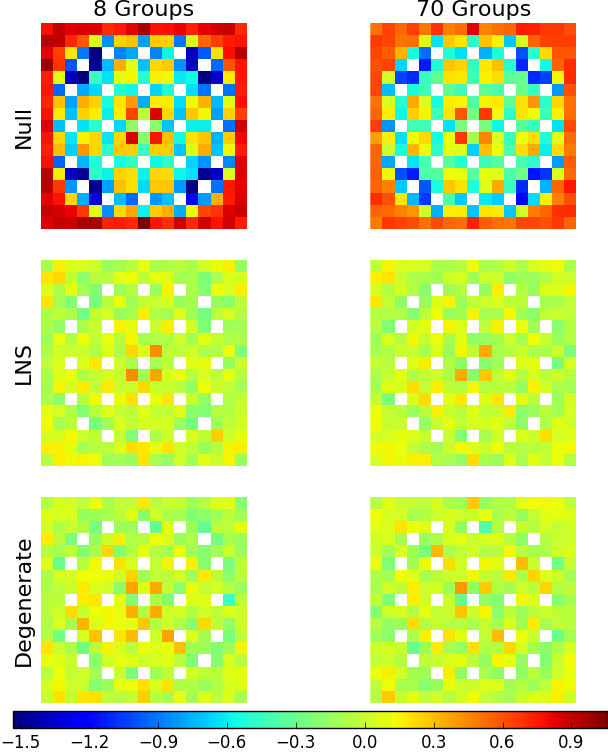
\includegraphics[width=\linewidth]{figures/patterns/lns/assm-16/capt-err}
\vspace{2mm}
\caption[U-238 capture rate errors for a 1.6\% enriched assembly]{U-238 capture rate percent relative errors errors for a 1.6\% enriched assembly with \ac{LNS} spatial homogenization.}
\label{fig:chap9-assm-1.6-lns-capt-err}
\end{figure}

\clearpage

\begin{figure}[h!]
\centering
\includegraphics[width=\linewidth]{figures/patterns/lns/assm-31/capt-err}
\vspace{2mm}
\caption[U-238 capture rate errors for a 3.1\% enriched assembly]{U-238 capture rate percent relative errors errors for a 3.1\% enriched assembly with \ac{LNS} spatial homogenization.}
\label{fig:chap9-assm-3.1-lns-capt-err}
\end{figure}

\clearpage

\begin{figure}[h!]
\centering
\includegraphics[width=\linewidth]{figures/patterns/lns/assm-31-20BPs/capt-err}
\vspace{2mm}
\caption[U-238 capture rate errors for a 3.1\% enriched assembly with 20 BPs]{U-238 capture rate percent relative errors errors for a 3.1\% enriched assembly with 20 \acp{BP} with \ac{LNS} spatial homogenization.}
\label{fig:chap9-assm-3.1-20BPs-lns-capt-err}
\end{figure}

\clearpage

\begin{figure}[h!]
\centering
\includegraphics[width=\linewidth]{figures/patterns/lns/2x2/capt-err}
\vspace{2mm}
\caption[U-238 capture rate errors for a 2$\times$2 colorset]{U-238 capture rate percent relative errors errors for a 2$\times$2 colorset with \ac{LNS} spatial homogenization.}
\label{fig:chap9-2x2-lns-capt-err}
\end{figure}

\clearpage

\begin{figure}[h!]
\centering
\includegraphics[width=\linewidth]{figures/patterns/lns/reflector/capt-err}
\vspace{2mm}
\caption[U-238 capture rate errors for a 2$\times$2 colorset with a reflector]{U-238 capture percent relative errors rate errors for a 2$\times$2 colorset with \ac{LNS} spatial homogenization.}
\label{fig:chap9-reflector-lns-capt-err}
\end{figure}

\clearpage

\begin{figure}[h!]
\centering
\includegraphics[width=\linewidth]{figures/patterns/lns/full-core/capt-err-null}
\vspace{2mm}
\caption[U-238 capture rate errors for \ac{BEAVRS} with null homogenization]{U-238 capture rate absolute errors for the 2D quarter core \ac{BEAVRS} model with null spatial homogenization.}
\label{fig:chap9-full-core-capt-err-null}
\end{figure}

\clearpage

\begin{figure}[h!]
\centering
\includegraphics[width=\linewidth]{figures/patterns/lns/full-core/capt-err-lns}
\vspace{2mm}
\caption[U-238 capture rate absolute errors for \ac{BEAVRS} with LNS homogenization]{U-238 capture rate absolute errors for the 2D quarter core \ac{BEAVRS} model with \ac{LNS} spatial homogenization.}
\label{fig:chap9-full-core-capt-err-lns}
\end{figure}

\clearpage

\begin{figure}[h!]
\centering
\includegraphics[width=\linewidth]{figures/patterns/lns/full-core/capt-err-degenerate}
\vspace{2mm}
\caption[U-238 capture rate absolute errors for \ac{BEAVRS} with degenerate homogenization]{U-238 capture rate absolute errors for the 2D quarter core \ac{BEAVRS} model with degenerate spatial homogenization.}
\label{fig:chap9-full-core-capt-err-degenerate}
\end{figure}

%\begin{figure}[h!]
%\centering
%\begin{subfigure}{.5\textwidth}
%  \centering
%  \includegraphics[width=0.9\linewidth]{figures/patterns/lns/full-core/capt-err-null}
%  \caption{}
%  \label{fig:chap9-full-core-null}
%\end{subfigure}%
%\begin{subfigure}{.5\textwidth}
%  \centering
%  \includegraphics[width=0.9\linewidth]{figures/patterns/lns/full-core/capt-err-null-magnitude}
%  \caption{}
%  \label{fig:chap9-full-core-null-magnitude}
%\end{subfigure}
%\begin{subfigure}{.5\textwidth}
%  \centering
%  \includegraphics[width=0.9\linewidth]{figures/patterns/lns/full-core/capt-err-lns}
%  \caption{}
%  \label{fig:chap9-full-core-lns}
%\end{subfigure}%
%\begin{subfigure}{.5\textwidth}
%  \centering
%  \includegraphics[width=0.9\linewidth]{figures/patterns/lns/full-core/capt-err-lns-magnitude}
%  \caption{}
%  \label{fig:chap9-full-core-lns-magnitude}
%\end{subfigure}
%\begin{subfigure}{.5\textwidth}
%  \centering
%  \includegraphics[width=0.9\linewidth]{figures/patterns/lns/full-core/capt-err-degenerate}
%  \caption{}
%  \label{fig:chap7-pin-1.6}
%\end{subfigure}%
%\begin{subfigure}{.5\textwidth}
%  \centering
%  \includegraphics[width=0.9\linewidth]{figures/patterns/lns/full-core/capt-err-degenerate-magnitude}
%  \caption{}
%  \label{fig:chap7-pin-crgt}
%\end{subfigure}
%\caption[U-238 capture rate errors for the \ac{BEAVRS} quarter core model]{U-238 capture percent relative errors rate errors for the \ac{BEAVRS} quarter core model with \ac{LNS} spatial homogenization.}\label{fig:chap9-full-core-lns-capt-err}
%\end{figure}

%\clearpage


%%%%%%%%%%%%%%%%%%%%%%%%%%%%%%%%%%%%%%%%%%%%%%%%%%%%%%%%%%%%%%%%%%%%%%%%%%%%%%%
\section{MGXS Convergence Rate Analysis}
\label{sec:chap9-convergence}

first paragraph: 
-Fig.~\ref{fig:chap9-converge}
  -batch-wise percentage change for \ac{MGXS} with null, degenerate and \ac{LNS} spatial homogenization
  -explain what ``batch-wise change'' means
-\ac{MGXS} for null changes the least from batch to batch
  -track density in each tally volume (in this case, all pins taken together) is greatest
-\ac{MGXS} for degenerate changes the most from batch to batch
  -track density in each tally volume (in this case, each unique fuel pin instance) is least
-\ac{MGXS} for \ac{LNS} changes less than degenerate but more than null
  -track density is in between since \ac{MGXS} are averaged across groups of like fuel pin instance

second paragraph: key takeaways
-convergence rate (slope) is same for all schemes
-averaging across pins shifts convergence curves to right
-the size/magnitude of the leftward shift depends on the number of pins being averaged across
-hence, the more pins we can average across, the faster we can compute \ac{MGXS} with \ac{MC}

third paragraph: segue into next chapter
-goal should be to best identify groups of pins with like \ac{MGXS}
-\ac{LNS} was used as one scheme
  -demonstrated promise for simple benchmarks
  -illustrated shortcomings for benchmarks with complicated heterogeneties
    -assembly-assembly and assembly-reflector interfaces
  -algorithm could be tweaked to pick up on these effects
    -customizations highly reactor dependent - NOT reactor agnostic
-would be nice to identify adequate pin groupings directly from structural patterns in the \ac{MGXS} data
-will do this in the following chapter

\begin{figure}[h!]
\centering
\begin{subfigure}{.87\textwidth}
  \centering
  \includegraphics[width=\linewidth]{figures/patterns/convergence/assm-16/assm-16-capt}
  \caption{}
  \label{fig:chap9-assm-16-converge}
\end{subfigure}
\begin{subfigure}{.87\textwidth}
  \centering
  \includegraphics[width=\linewidth]{figures/patterns/convergence/full-core/16-enr-capt}
  \caption{}
  \label{fig:chap9-reflector-converge}
\end{subfigure}
\caption[Convergence of pin-wise U-238 capture MGXS]{The batch-wise change of pin-wise U-238 capture \ac{MGXS} (group 27 of 70) for 1.6\% enriched fuel pins in a single assembly (a) and the quarter core \ac{BEAVRS} model (b). The convergence of both the maximum and mean absolute percent change are shown for the degenerate and \ac{LNS} homogenization schemes.}
\label{fig:chap9-converge}
\end{figure}


SUMMARY BOXES!!!
